%%%%%%%%%%%%%%%%%%%%%%%%%%%%%%%%%%%%%%%%%%%%%%%%%%%%%%%%%%%%%%%%%%%%%%%%%%
%
% StEvent - User Guide and Reference Manual -- LaTeX Source
%
% $Id: StEvent.tex,v 1.19 1999/04/19 17:37:21 genevb Exp $
%
% Author: Thomas Ullrich, March 1999
%
%%%%%%%%%%%%%%%%%%%%%%%%%%%%%%%%%%%%%%%%%%%%%%%%%%%%%%%%%%%%%%%%%%%%%%%%%%
%
% Notes to the authors:
%
% - A template for a class reference is at the end of this file.
% - Wrap all names functions with \name{}
% - All code, examples, prototypes in \verb+ ... +\\
%   or /begin{verbatim} ... \end{verbatim}
% - Use \StEvent if you refer to the package itself (not the class)
%
% This file is best edit with xemacs and the 'Function' package loaded.
%
%%%%%%%%%%%%%%%%%%%%%%%%%%%%%%%%%%%%%%%%%%%%%%%%%%%%%%%%%%%%%%%%%%%%%%%%%%
%
% $Log: StEvent.tex,v $
% Revision 1.19  1999/04/19 17:37:21  genevb
% Updated vertex documentation
%
% Revision 1.20  1999/04/19 20:46:41  ullrich
% Mods to StHit (virtual)
%
% Revision 1.19  1999/04/19 17:37:21  genevb
% Updated vertex documentation
%
% Revision 1.18  1999/04/13 23:27:23  genevb
% Slightly refined vertex code, updated V0, Xi vertex documentation
%
% Revision 1.17  1999/04/08 15:27:52  ullrich
% Added description of PID classes
%
% Revision 1.16  1999/03/31 19:03:50  ullrich
% Corrected typos in UML appendix
%
% Revision 1.15  1999/03/30 19:41:17  ullrich
% Added Torres 'how to' tutorial. Text pasted from web.
%
% Revision 1.14  1999/03/30 19:11:53  genevb
% Correct typo from last change
%
% Revision 1.13  1999/03/30 18:54:15  genevb
% Add Xi documentation
%
% Revision 1.12  1999/03/26 08:10:29  ullrich
% Corrected typos, text smoothed.
%
% Revision 1.11  1999/03/25 22:10:54  ullrich
% Added brief introduction to UML (appendix A).
%
% Revision 1.10  1999/03/25 14:05:41  ullrich
% Improved some explanation. More index entries.
%
% Revision 1.9  1999/03/24 19:03:43  ullrich
% Fixed bug in UML figure numbers.
%
% Revision 1.8  1999/03/23 23:10:05  ullrich
% Added latest changes to StEvent.
%
% Revision 1.7  1999/03/19 17:22:44  ullrich
% Save current version.
%
% Revision 1.6  1999/03/16 00:49:23  ullrich
% Check in current status
%
% Revision 1.5  1999/03/12 21:55:13  ullrich
% Save current status.
%
% Revision 1.4  1999/03/11 21:10:28  ullrich
% Update
%
% Revision 1.3  1999/03/11 16:11:19  ullrich
% Snapshot of work in progress.
%
% Revision 1.2  1999/03/09 21:49:25  ullrich
% Added class reference for EMC hits. New examples.
%
% Revision 1.1  1999/03/09 17:28:28  ullrich
% Initial Revision
%
% Revision 2.33  2000/05/22 22:04:07  ullrich
% Removed StRichPixelCollection ref section and added description
% of new RICH methods to class StEvent.
%
% Revision 2.45  2000/08/23 03:14:07  ullrich
% Improved (corrected) explanation of return value
% of chi2 methods of StVertex and StTrackFitTraits.
%
% Revision 2.44  2000/08/17 00:36:31  ullrich
% Added description of StTptTrack.
%
% Revision 2.43  2000/08/17 01:18:02  ullrich
% Fixed wrong description of StZtbTriggerDetector::adc().
%
% Revision 2.42  2000/07/13 12:47:07  ullrich
% Added ZDC info provided by Clemens
%
% Revision 2.41  2000/06/29 18:00:37  ullrich
% Better description of StCtbTriggerDetector.
%
% Revision 2.40  2000/06/22 18:18:33  ullrich
% Fixed problem with page numbering. Increased textheight.
%
% Revision 2.39  2000/06/21 22:55:42  ullrich
% Added StEventInfo to ref section. Updated StEvent.
%
% Revision 2.38  2000/06/07 09:44:20  ullrich
% Modified StHit ref section.
%
% Revision 2.37  2000/06/01 21:36:17  ullrich
% Added new method flag() to StHit description.
%
% Revision 2.36  2000/06/01 16:46:23  ullrich
% Mods (add text) in StTrack and StTrackDetectorInfo.
%
% Revision 2.35  2000/05/31 14:26:26  lasiuk
% Add RICH classes and descriptions
%
% Revision 2.32  2000/05/17 17:20:01  ullrich
% Updates and improved description of StTrackTopologyMap.
% Revision 2.31  2000/05/16 13:22:39  ullrich
% More details on the second chi2 value in StTrackFitTraits.
%
% Revision 2.30  2000/05/09 11:09:30  ullrich
% Updated section on StMwcTriggerDetector and StCtbTriggerDetector.
%
% Revision 2.29  2000/04/26 21:01:44  ullrich
% Removed text for obsolete StBrowsableEvent.
%
% Revision 2.28  2000/04/20 13:31:25  ullrich
% Added description of changes to StTrackDetectorInfo.
%
% Revision 2.27  2000/04/10 19:59:34  genevb
% StRoot/StEvent/doc/tex/
%
% Revision 2.26  2000/03/30 16:55:38  ullrich
% Modified reference section for StTrack::key().
%
% Revision 2.25  2000/03/29 16:55:48  ullrich
% Added reference section and emprt user guide page for StL3Trigger.
%
% Revision 2.24  2000/03/23 18:30:50  ullrich
% Added new EMC classes to reference section.
%
% Revision 2.23  2000/03/08 14:27:45  ullrich
% Added description of new method of StVertex.
%
% Revision 2.22  2000/03/02 12:40:40  ullrich
% Added description of modified StTpcDedxPidAlgorithm
%
% Revision 2.21  2000/02/28 19:37:26  ullrich
% Added the hypperref package to add bookmarks and hyperlinks
% tp pdf documents.
%
% Revision 2.20  2000/02/24 13:25:12  ullrich
% Added RICH and EMC to the reference section. Created
% (empty) section for EMC and RICH in User Guide.
  {\LARGE $ $Revision: 1.19 $ $}  \\[5mm] % replaced by cvs with current revision
  {\LARGE $ $Date: 1999/04/19 17:37:21 $ $}  % replaced by cvs with current revision
%
% Revision 2.18  2000/02/11 16:23:45  ullrich
% Add info on order in which primary vertices are stored
  {\LARGE User Guide and Reference Manual}\\[2cm]
  {\LARGE $ $Revision: 1.19 $ $}  \\[5mm] % replaced by cvs with current revision
  {\LARGE $ $Date: 1999/04/19 17:37:21 $ $}  % replaced by cvs with current revision
% Added Helens description of iflag (see StTrack::flag()).
%
% Revision 2.16  2000/01/27 18:38:30  ullrich
% Fixed typo in units for curvature.
%
% Revision 2.15  2000/01/12 10:45:31  ullrich
% Fixed error (underscore in text).
%
% Revision 2.14  2000/01/11 16:31:56  ullrich
% Regular update.
%
%%%%%%%%%%%%%%%%%%%%%%%%%%%%%%%%%%%%%%%%%%%%%%%%%%%%%%%%%%%%%%%%%%%%%%%%%%
\documentclass[twoside]{article}

\parindent 0pt
\parskip 6pt
%    User Guide
\advance\textwidth by 80pt%
\advance\evensidemargin by -80pt%

\part{User Guide}
\clearpage

%%%%%%%%%%%%%%%%%%%%%%%%%%%%%%%%%%%%%%%%%%%%%%%%%%%%%%%%%%%%%%%%%%%%

\section{Introduction}

\StEvent\footnote{The name ``StEvent'' is somewhat misleading since it
    is \textit{(i)} the name of the package and \textit{(ii)} the name
    of a class.  We therefore write \StEvent\ when we refer to the
    package and \name{StEvent} for the class.} is an object oriented
framework to access, manipulate and analyze STAR DSTs. It consist of a
set of C++ classes which are connected in a tree like structure. The
top class is \name{StEvent} which represents also the single entry
point to the whole tree. All what is needed to access every instance
in the tree and navigate freely through the structure is a pointer to
\name{StEvent}. This pointer can be obtained from the
\name{StEventReaderMaker} which is explained in detail in
sec.~\ref{sec:howto}.

Although \StEvent\ benefits from the flexibility of the OO design it
is strongly constraint by the existing DST model where the data is
stored in flat tables and references are maintained by keys into
referring tables.  When \StEvent\ is set up the content of the tables
is mapped to the OO model and keys are replaced by associations
between classes through pointer and references.

\begin{figure}[htb]
    \begin{center}
        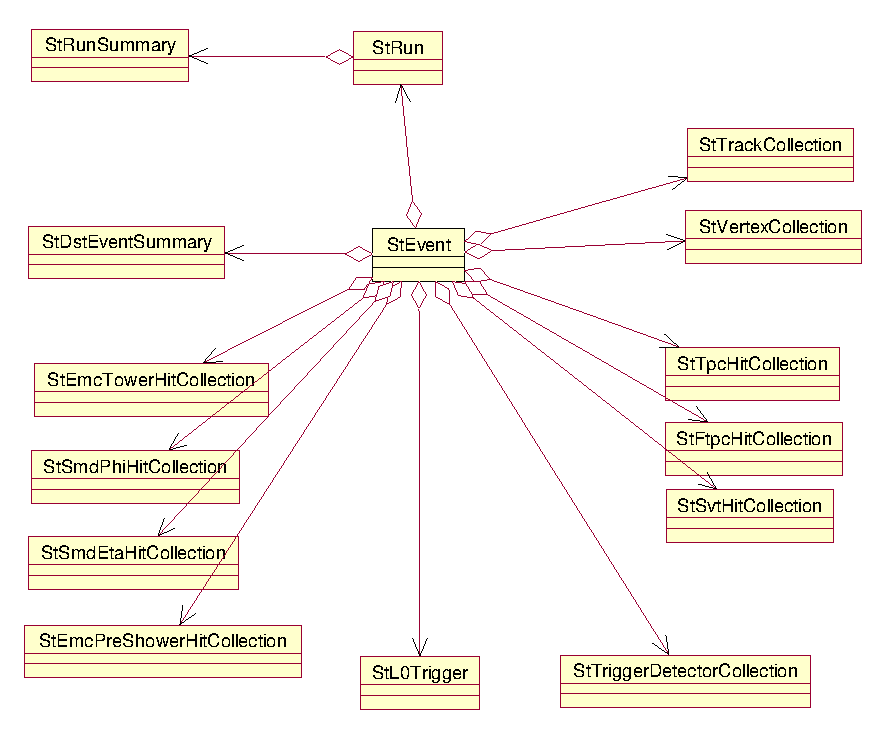
\includegraphics[width=0.95\textwidth]{umlForEvents.eps}
    \caption{UML diagram showing the top class \name{StEvent} and its
        directly related classes.}
    \label{fig:umlForEvents}
\end{center}
\end{figure}
\usepackage{graphicx}
Overall the design of \StEvent\ is fairly simple which reflects the
fact that the package is strongly focused on simple data access and
navigation.  In order to give an overview without going to much in
detail Fig.~\ref{fig:umlForEvents}-\ref{fig:umlForVertices} show some
basic class diagrams using the Unified Modelling Language UML (see
Appendix~\ref{sec:introUML} for a brief introduction to UML).

Fig.~\ref{fig:umlForEvents} shows an UML class diagram \index{UML}
which illustrates the first layer of classes directly connected to
\name{StEvent}. Most notably are the collections for hits, tracks and
vertices. Each event has a run associated with it which is described
by the \name{StRun} class. \\
A more simple structure of concrete classes is depicted in
Fig.~\ref{fig:umlForHits}. Shown is the relations between the various
hit classes: the base class \name{StHit} and the three derived classes
for hits in the TPC, FTPC and SVT. The arrow from \name{StHit} to the
three vector class \name{StThreeVector} indicates a 'has a'
relationship, since the actual position in xyz is stored in a data
member of type \name{StThreeVector}.
\usepackage{amsmath}
\begin{figure}[htb]
% Typographic Conventions
    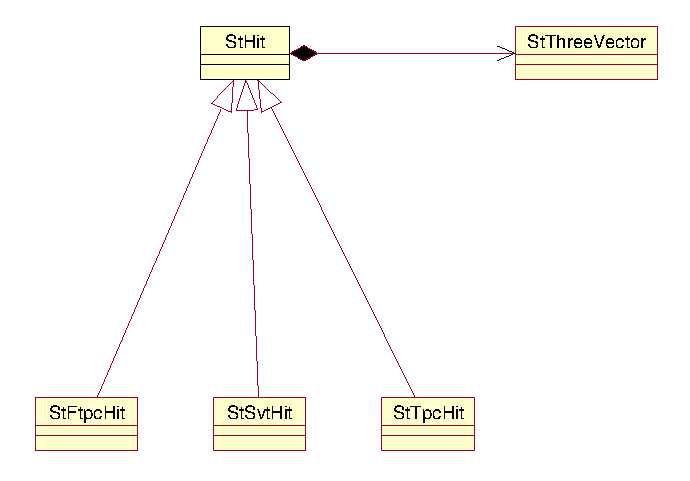
\includegraphics[height=0.4\textheight]{umlForHits.eps}
    \caption{Dependencies for the TPC, FTPC and SVT hit classes.}
    \label{fig:umlForHits}
\newcommand{\StEvent}{\textsf{StEvent}}

%%%%%%%%%%%%%%%%%%%%%%%%%%%%%%%%%%%%%%%%%%%%%%%%%%%%%%%%%%%%%%%%%%%%
Fig.~\ref{fig:umlForTracks} shows a more complex diagram which
describes a global track (\name{StGlobalTrack}) and its dependencies.
Global tracks are the essential backbone of the data model. They
contain references to their hits in the various detectors and keep
track of their start and stop vertices.  (see
fig.~\ref{fig:umlForVertices}).

\begin{figure}[htb]
    \begin{center}
        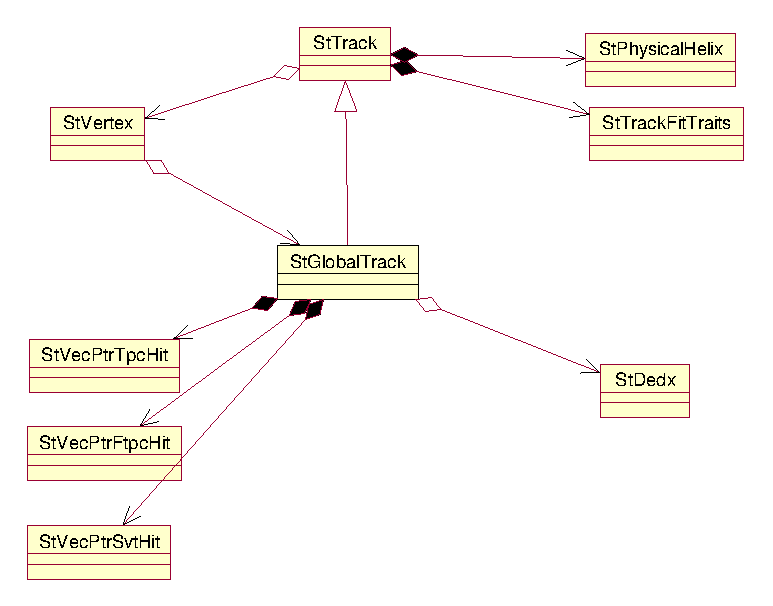
\includegraphics[height=0.4\textheight]{umlForTracks.eps}
    \caption{Data model for \name{StGlobalTrack} and related classes.}
    \label{fig:umlForTracks}
\end{center}
\end{figure}

The dependencies of the various kinds of vertices is shown in
Fig.~\ref{fig:umlForVertices} on page \pageref{fig:umlForVertices}.
The base class \name{StVertex} is used for most of the common types of
vertices while more specialized classes, e.g.~\name{StXiVertex},
derived from it have a more complex design reflecting their higher
degree of specialization.

\begin{figure}[htb]
    \begin{center}
        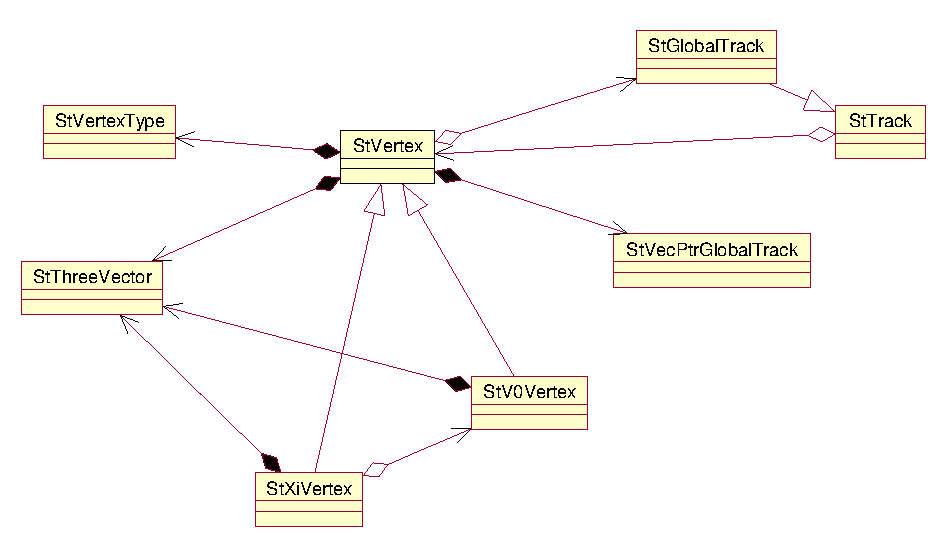
\includegraphics[height=0.4\textheight]{umlForVertices.eps}
    \caption{Data model for the vertices and related classes in \StEvent .}
    \label{fig:umlForVertices}
\end{center}
\end{figure}

%
% Define multiline labels for class reference
%

\section{How to read this document}

This document is intended to serve the advanced users as well as
beginners. It is therefore divided in two parts, a user guide and a
reference manual. In the first part we rather concentrate on basic
questions and provide guidance to get started.  The reference section
provides information on all available classes, their member functions
and related operators. Each class reference contains one or more
examples which demonstrates some features of the class and how to use
it.

New users should \textbf{not} start with the Reference section. It is
meant as a lookup when specific information is needed. Beginners
should study the User Guide and should make themself familiar only
with those classes they will encounter more frequently: \name{StEvent}
(sec.~\ref{sec:StEvent}), \name{StGlobalTrack}
(sec.~\ref{sec:StGlobalTrack}), \name{StVertex}
(sec.~\ref{sec:StVertex}), and \name{StTpcHit}
(sec.~\ref{sec:StVertex}).  Reading and understanding the various
examples certainly is the best way to get started. Note, however, that
the examples shown throughout this guide are often not complete and
are not guaranteed to compile. Their only purpose is to illustrate a
specific feature and not to provide a fully functional programming
unit.

  {\LARGE $ $Date: 1999/04/19 17:37:21 $ $}  % replaced by cvs with current revision
     \advance\leftmargin by \labelsep%
\section{Further documentation}
\label{sec:furtherdoc}

\StEvent\ makes use of various classes from the StarClassLibrary (SCL).
To obtain the SCL documentation perform the following steps:
\begin{enumerate}
  \item Obtain an \name{afs} token: \name{klog -cell rhic}.
  \item Make sure \name{\$CVSROOT} is set properly:\\
    (i.e.~\name{CVSROOT = /afs/rhic/star/packages/repository})
  \item Check-out the SCL into your current working directory:\\
    \name{cvs checkout StRoot/StarClassLibrary}
  \item Go to the directory containing the documentation:\\
    \name{cd StRoot/StarClassLibrary/doc/tex}
  \item Create the PostScript document \name{StarClassLibrary.ps}:\\
    \name{make}
\end{enumerate}
\index{SCL} \index{StarClassLibrary}
  {\end{list}}
%%%%%%%%%%%%%%%%%%%%%%%%%%%%%%%%%%%%%%%%%%%%%%%%%%%%%%%%%%%%%%%%%%%%
  {\Large\bf STAR Offline Library Long Writeup}
\section{Getting \StEvent\ Sources}  \index{Getting StEvent sources}
  \hfill\mbox{}\\[3cm]
The \StEvent\ package is part of the official STAR software distribution
and is therefore present in the actual STAR software releases. To access
the complete source code proceed as follows:

\StEvent\ is under {\bf CVS} control at BNL.  It can
be accessed via \name{afs}: \index{afs} \index{CVS} \index{CVSROOT}
\begin{enumerate}
  \item Obtain an \name{afs} token: \name{klog -cell rhic}.
  \item Make sure \name{\$CVSROOT} is set properly:\\
    (i.e.~\name{CVSROOT = /afs/rhic/star/packages/repository})
  \item Check-out package into your current working directory:\\
    \name{cvs checkout StRoot/StEvent}
\end{enumerate}

%%%%%%%%%%%%%%%%%%%%%%%%%%%%%%%%%%%%%%%%%%%%%%%%%%%%%%%%%%%%%%%%%%%%

\section{Coding Standards}
\index{Coding Standards}

\StEvent\ follows the STAR coding guidelines as described on the
STAR web page: \\
http://rsgi01.rhic.bnl.gov/STAR/html/comp\_l/train/standards.html.\\
All developers are encouraged to follow this small set of rules in
order to create a homogeneous and coherent interface style.  Here we
summarize the most relevant one concerning the programmable interface:
\begin{itemize}
\item all classes, enumerations and functions start with the prefix
    \textbf{St}
\item all member function start with a lowercase letter
\item header files have the extension \textbf{.hh}, source files have
    the extension\textbf{ .cc}
\item the use of underscores in names is discouraged
\item classes, methods, and variables have self-explanatory English
    names and first letter capitalization to delineate words
\end{itemize}

In addition \StEvent\ defines a few rules which ease its usage
\begin{itemize}
\item methods (member functions) which return a certain object have
    the same name as the referring object, i.e., without a preceding
    \name{get} prefix \\ (as in \name{StEvent::primary\-Vertex()})
\item methods which assign a value to a data member (or members) carry
    the prefix \name{set} followed by the name of the member (as in \name{StEvent::set\-Primary\-Vertex()}).
\item integer variables which serve as counter or indices and never
    can take negative values are consistently of declared as
    \name{unsigned}.
\item the \name{const} identifier is used wherever possible. Remember:
    \begin{itemize}
    \item const member functions are guaranteed to not alter data
        member
    \item const arguments are guaranteed to not be modified by the
        function
    \item const return values cannot be modified
    \end{itemize}
    \name{const}'ness implies a slightly higher compile time overhead
    but a faster execution time.
\item Objects which are returned by pointer are not guaranteed to
    exist in which case a null pointer is returned. It is users
    responsibility to check for the return value and make sure the
    pointer is valid (non-zero) before she dereference it.  Objects
    which are granted to exist are returned by reference or by value.
\end{itemize}

%%%%%%%%%%%%%%%%%%%%%%%%%%%%%%%%%%%%%%%%%%%%%%%%%%%%%%%%%%%%%%%%%%%%

\section{How to use it: doEvents.C and StEventReaderMaker}
% text from Torres tutorial web page
\label{sec:howto}
\index{doEvents.C}
\index{StEventReaderMaker}
\index{StAnalysisMaker}
\index{root4star}
\index{ROOT files}
\index{XDF files}
The procedure starting from scratch to run the provided StEvent usage
example is
\begin{verbatim}
    stardev
    mkdir workdir
    cd workdir
    root4star doEvents.C
\end{verbatim}

This will run \name{\$STAR/StRoot/macros/doEvents.C} which runs a
chain consisting of two makers:
\begin{description}
\item[\name{StEventReaderMaker}:] Read events from DST input files (XDF
    files or ROOT files; the file is handled appropriately based on
    file type) and load StEvent
\item[\name{StAnalysisMaker}:] Pick up the StEvent event and analyze it
    (incorporates a few simple examples)
\end{description}
It runs the chain on either a single file or all files under a
specified root directory (see doEvents.C for details), eg. example
invocations are
\begin{verbatim}
.x doEvents.C(10,"-","/afs/rhic/star/strange/genevb/year1a_90evts_dst.xdf")
     processes 10 events from the specified file

.x doEvents.C(9999,"/disk00000/star/auau200/hijing135/"," ")
     processes all events from all files found recursively under the
     specified directory
\end{verbatim}
The multiple-files feature currently only works for XDF files.  To
play with it yourself you can pick up StAnalysisMaker and play with it
or use it as a template for a Maker of your own that works with
StEvent:
%    Introduction
%
    mkdir StRoot/StMyAnalysisMaker
    cp $STAR/StRoot/StAnalysisMaker/* StRoot/StMyAnalysisMaker/
    [edit]
    makel -C StRoot/StMyAnalysisMaker
    cp $STAR/StRoot/macros/doEvents.C ./  (and edit to use your maker)
    root4star doEvents.C
\end{verbatim}
Using some XDF files you will see messages about changed table
structures. The DST tables themselves are not affected.


%%%%%%%%%%%%%%%%%%%%%%%%%%%%%%%%%%%%%%%%%%%%%%%%%%%%%%%%%%%%%%%%%%%%
                             kOtherVtxId};
\section{Units}
\index{units} \index{system of units}
enum StDedxMethod           {kUndefinedMethodId,

All quantities in \StEvent\ are stored using the official STAR units:
cm, GeV and Tesla.  In order to maintain a coherent system of units it
is recommended to use the definitions in \name{SystemOfUnits.h} from
the StarClassLibrary. They allow to 'assign' a unit to a given
variable by multiplying it with a constant named accordingly
(centimeter, millimeter, kilometer, tesla, MeV, ...).  The value of
the constants is thus that the result after the multiplication follows
always the STAR system of units.

                             tpcOther,
{\footnotesize
                             ftpcConformal,
                             svtTpcSvm,
                             svtTpcEst,
                             svtTpcPattern};

enum StRichPidFlag          {eNoMip,
                             eFastEnough,
                             eLightOnPadPlane};
\end{verbatim}

Note that often the enumeration type names (e.g. \texttt{StTrackType})
are used as argument types. The strong C++ type checking rules ensures
the proper use of the enumeration constants already during
compilation.

Another important set of constants should be mentioned here as well,
namely the physical constants defined in \texttt{PhysicalConstants.h}.
There are too many to be listed here but you should make yourself
familiar with what constants are available. You will find the header
file in the \name{StarClassLibrary} (see Sec.~\ref{sec:furtherDoc}).
\index{StarClassLibrary} In order to define the units of the various
physical constants another set of constants defined in
\texttt{SystemOfUnits.h} is used (also from \name{StarClassLibrary}).
The latter is described in section \ref{sec:units}.

\subsection{Conventions}
\index{conventions}
}%footnotesize
\label{sec:conventions}
{\footnotesize

\subsubsection{Numbering Scheme}
\label{sec:conventionsNumbering}

All numbering follows \emph{strictly} the C/C++ convention, i.e. the
first element in an array has the index 0. This is valid for all
container, collections and lists. Here it is important to remember
that many (but not all) official STAR numbering schemes start counting
at 1.  Examples are TPC sectors and padrows, SVT barrels, layers, ladders and
wafers. Do not forget to subtract 1 when using this scheme for
addressing elements in a container.

TPC, SVT and FTPC hits return their hardware address in STAR units.
In order to select the hit container in which a hit \texttt{h} is
stored you must write:
}%footnotesize
Further documentation can be found in the StarClassLibrary manual
(see sec.~\ref{sec:furtherdoc}).
\end{verbatim}
%%%%%%%%%%%%%%%%%%%%%%%%%%%%%%%%%%%%%%%%%%%%%%%%%%%%%%%%%%%%%%%%%%%%

\section{Known Problems} \index{known problems (\StEvent)}

\StEvent\ is continuously improved. In certain cases it might happen
that the documentation isn't up-to-date. In these cases the header
file should be visited.

Although \StEvent\ is updated frequently it might happen that it lacks
means of accessing some specific DST information since the content of
the DST changes considerably in time. We expect a more stable
situation as soon as experimental data comes in and the DST format
gets better defined.  \index{DST files}

\clearpage

%%%%%%%%%%%%%%%%%%%%%%%%%%%%%%%%%%%%%%%%%%%%%%%%%%%%%%%%%%%%%%%%%%%%
%
%    Reference Manual
%
%%%%%%%%%%%%%%%%%%%%%%%%%%%%%%%%%%%%%%%%%%%%%%%%%%%%%%%%%%%%%%%%%%%%
\part{Reference Manual}
\clearpage

%%%%%%%%%%%%%%%%%%%%%%%%%%%%%%%%%%%%%%%%%%%%%%%%%%%%%%%%%%%%%%%%%%%%

\section{Global Constants, Enumerations and Definitions}

In addition to the constants defined in the two header files
\index{StarClassLibrary} \name{SystemOfUnits.h} and
\name{PhysicalConstants.h} which are part of the StarClassLibrary
\StEvent\ defines a set of enumeration types in
\name{StEnumerations.hh}. The types defined therein are used
throughout \StEvent .

\subsection{Enumeration Types}
\index{enumerations}
\label{sec:StEnumerations}
    \begin{center}
\item[Summary]
  Global Enumeration types.
\end{figure}

\item[Synopsis]
  \verb+#include "StEnumerations.hh"+ \\

typedef short          Short_t;     //Signed Short integer 2 bytes
\item[Description]
    \index{StBeamDirection|textbf}
    \index{StBeamPolarizationAxis|textbf}
    \index{StVertexType|textbf}
    \index{StTrackSign|textbf}
    The header file does not only define the enumerations and their values
    but also the \textit{type} of the enumeration set. This allows the
    different enumerations to be used as argument types where the strong C++ type
    checking rules ensures the proper use of the enumeration constants already
    during compilation.

    \verb+enum StBeamDirection {east, west};+\\
typedef double         Double_t;    //Float 8 bytes
    \verb+enum StBeamPolarizationAxis {sideways, vertical, longitudinal};+\\

    \verb+enum StVertexType {undefined, primary, kink,+\\
    \verb+                   twoBody, threeBody, nBody,+\\
    \verb+                   pileUpPrimary, V0, Xi};+\\

    \verb+enum StTrackSign {negativeTrack, positiveTrack};+\\

    Please remember that C++ starts the enumeration with 0 (zero) unless
    explicitly given otherwise. The definition of enumeration types allows
    to define the following function:\\
    \verb+myfunc(StBeamDirection d);+\\
    Any argument value other than \name{east} or \name{west} causes a compile
    time error. (Note, that even the integer values 0 and 1 would fail to compile.)

\end{Entry}

for (int i=0; i<theHits.size(); i++) {

\section{Collections and Iterators}
\label{sec:collections}
\index{collection|textbf}
\index{iterator}
\index{StEmcPreShowerHitCollection|textbf}
\index{StEmcTowerHitCollection|textbf}
\index{StFtpcHitCollection|textbf}
\index{StSmdEtaHitCollection|textbf}
\index{StSmdPhiHitCollection|textbf}
\index{StSvtHitCollection|textbf}
\index{StTpcHitCollection|textbf}
\index{StTrackCollection|textbf}
\index{StVecCtbCounter|textbf}
\index{StVecMwcSector|textbf}
\index{StVecPtrFtpcHit|textbf}
\index{StVecPtrGlobalTrack|textbf}
\index{StVecPtrSvtHit|textbf}
\index{StVecPtrTpcHit|textbf}
\index{StVecVpdCounter|textbf}
\index{StVecZdcSegment|textbf}
\index{StVertexCollection|textbf}
\index{StVecTH1F|textbf}
\index{StVecTH2F|textbf}

\StEvent\ defines various collection classes and their referring
iterators.  They differ in type -- collecting objects by pointer or by
value -- and by the underlying collection classes (sequence container, linked list, maps).
The latter, however, is always encapsulated in the implementation. All
collection classes have a common interface which follows the C++
standard, i.e.~the Standard Template Library (STL) \index{STL}. Most
containers are actually implemented as STL containers although this
might change in future. In case the container will get replaced with more
specialized versions we will
make sure the replacement provides methods which are compatible with those
of the standard to maintain the integrity of existing code.

All container are guaranteed to provide at least the following member functions:
\name{size()}, \name{begin()}, \name{end()}.  Most collection in
\StEvent\ have a referring iterator defined (see table \ref{tab:stcoll})
which is declared in the same header file as the
corresponding collection.

In order to keep your code independent of the underlying container
types users are encouraged to use \textit{iterators} instead of
indices. The higher degree of flexibility allows to change containers
without changing the application code using them. The following
examples demonstrates this:

Given an arbitrary \StEvent\ collection \name{anyColl} of type \name{StAnyColl}
which holds objects of type
\name{obj} the following code is not guaranteed to work:
\begin{verbatim}
     for (int i=0; i<anyColl.size(); i++)
         obj = anyColl[i];
\end{verbatim}
It should be replaced by:
\begin{verbatim}
     StAnyCollIterator iter;
     for (iter = anyColl.begin(); iter != anyColl.end(); iter++)
         obj = *iter;
\end{verbatim}

\StEvent\ distinguishes two sorts of collection classes:
\begin{enumerate}
\item Collections of general importance which are accessible through
    the \name{StEvent} class itself, i.e., \name{StEvent} provides member functions
    which return pointer or references to them.  There names are
    composed of the name of the objects they hold and the word
    \name{Collection}.  All containers of this type are listed in
    table \ref{tab:stcoll}.  The hold the essential objects as hits,
    tracks and vertices.

\item Simple collection classes which are returned or used in various classes
    further down the tree.  Their naming scheme is different from
    the main collection classes. Without exception the
    underlying container is a sequence container, i.e., the
    \name{operator[]} can be used safely. Their names are all prefixed
    \name{StVec} or \name{StVecPtr} (in case the objects are collected
    via pointers) followed by the name of the object they collect. All
    available types are listed in table \ref{tab:stvec}
\end{enumerate}

\begin{table}[htb]
    \begin{center}
    \footnotesize\
    \begin{tabular}{|l|l|l|l|}
        \hline
        \textbf{Collection Class} & \textbf{Elements} & \textbf{Iterator} & \textbf{Header File} \\ \hline
\name{StEmcPreShowerHitCollection} & \name{StEmcPreShowerHit} & \name{StEmcPreShowerHitIterator} & \name{StEmcPreShowerHitCollection.hh}  \\ \hline
\name{StEmcTowerHitCollection}     & \name{StEmcTowerHit}     & \name{StEmcTowerHitIterator}     & \name{StEmcTowerHitCollection.hh}  \\ \hline
\name{StSmdEtaHitCollection}       & \name{StSmdEtaHit}       & \name{StSmdEtaHitIterator}       & \name{StSmdEtaHitCollection.hh}  \\ \hline
\name{StSmdPhiHitCollection}       & \name{StSmdPhiHit}       & \name{StSmdPhiHitIterator}       & \name{StSmdPhiHitCollection.hh}  \\ \hline
\name{StFtpcHitCollection}         & \name{StFtpcHit$*$}      & \name{StFtpcHitIterator}         & \name{StFtpcHitCollection.hh}  \\ \hline
\name{StSvtHitCollection}          & \name{StSvtHit$*$}       & \name{StSvtHitIterator}          & \name{StSvtHitCollection.hh}  \\ \hline
\name{StTpcHitCollection}          & \name{StTpcHit$*$}       & \name{StTpcHitIterator}          & \name{StTpcHitCollection.hh}  \\ \hline
\name{StTrackCollection}           & \name{StGlobalTrack$*$}  & \name{StTrackIterator}           & \name{StTrackCollection.hh}  \\
{}                                 & {}                       & \name{StTrackConstIterator}      & {}                     \\ \hline
\name{StVertexCollection}          & \name{StVertex$*$}       & \name{StVertexIterator}          & \name{StVertexCollection.hh}  \\ \hline
    \end{tabular}
    \caption{Main collection classes.}
    \label{tab:stcoll}
    \end{center}
\end{table}

\begin{table}[htb]
    \begin{center}
    \footnotesize\
    \begin{tabular}{|l|l|l|l|}
        \hline
        \textbf{Collection Class} & \textbf{Elements} & \textbf{Iterator} & \textbf{Header File} \\ \hline
\name{StVecCtbCounter}     & \name{StCtbCounter}   & \name{StVecCtbCounterIterator}     & \name{StVecCtbCounter.hh}  \\ \hline
\name{StVecMwcSector}      & \name{StMwcSector}    & \name{StVecMwcSectorIterator}     & \name{StVecMwcSector.hh}  \\ \hline
\name{StVecPtrFtpcHit}     & \name{StFtpcHit$*$}     & \name{StVecPtrFtpcHitIterator} & \name{StVecPtrFtpcHit.hh}  \\ \hline
\name{StVecPtrGlobalTrack} & \name{StGlobalTrack$*$} & \name{StVecPtrGlobalTrackIterator}     & \name{StVecPtrGlobalTrack.hh}  \\ \hline
\name{StVecPtrSvtHit}      & \name{StSvtHit$*$}      & \name{StVecPtrSvtHitIterator}  & \name{StVecPtrSvtHit.hh}  \\ \hline
\name{StVecPtrTpcHit}      & \name{StTpcHit$*$}      & \name{StVecPtrTpcHitIterator}  & \name{StVecPtrTpcHit.hh}  \\ \hline
\name{StVecVpdCounter}     & \name{StVpdCounter}   & \name{StVecVpdCounterIterator}     & \name{StVecVpdCounter.hh}  \\ \hline
\name{StVecZdcSegment}     & \name{StZdcSegment}   & \name{StVecZdcSegmentIterator}     & \name{StVecZdcSegment.hh}  \\ \hline
\name{StVecTH1F}     & \name{TH1F}   & \name{--}     & \name{StTHDefs.hh}  \\ \hline
\name{StVecTH2F}     & \name{TH2F}   & \name{--}     & \name{StTHDefs.hh}  \\ \hline
    \end{tabular}
    \caption{Utility collections classes based on sequence containers.}
    \label{tab:stvec}
    \end{center}
\end{table}

Note, that some collections contain objects by value other by pointer.
Container which collect objects by pointer or reference are also often
called \textit{polymorphic} container since they are not restricted to
collect objects of the base type only but of any type derived from
it. This is especially important when dereferencing the iterator to
access the objects in the collection.  For a \textit{by-value}
collection:
\begin{verbatim}
     StEmcPreShowerHitIterator iter;
     StEmcPreShowerHitCollection* hits =
                         event->emcPreShowerHitCollection();
     StEmcPreShowerHit *hit;
     for (iter = hits->begin(); iter != hits->end(); iter++)
         hit = iter;             // no dereference necessary
\end{verbatim}
But for a \textit{by-pointer} collection:
\begin{verbatim}
     StVertexIterator iter;
     StVertexCollection* vertices = event->vertexCollection();
     StVertex *vertex;
     for (iter = vertices->begin(); iter != vertices->end(); iter++)
         vertex = *iter;                         // dereference once
\end{verbatim}

Hint: Use pointers or references to collection elements wherever
possible.  Making local copies is often time- and memory-intensive.
For example the same code above but written as:
\begin{verbatim}
     StVertexIterator iter;
     StVertexCollection* vertices = event->vertexCollection();
     StVertex vertex;
     for (iter = vertices->begin(); iter != vertices->end(); iter++)
         vertex = **iter;                         // dereference twice
\end{verbatim}
invokes the \name{StVertex} assignment operator and creates a local copy.
This method is only useful if you intend to modify am object locally
but want to leave the original untouched.

\newpage

    assert(theHits[i]->wafer() == iwafer);

\section{Class Reference}
\index{StMeasuredPoint}
STAR CVS repository are described in alphabetic order.
\texttt{StMeasuredPoint} can be used wherever positions and errors
are what count. Take for an example a track fit. What you have to pass
reference section of a derived class. Always check the section(s)
of the base class(es) to get a complete overview on the available
are the coordinates and their weight which depends on the errors.
\end{verbatim}
Note that some constructors are omitted, especially the ones which
take tables as arguments. They are for nternal use only (even if
public).

Destructors, assignment operators and copy constructors are not
listed.  \name{Inline} declarations are omitted throughout the
documentation.

    \verb+#include "StTpcHitCollection.h"+\\
    \verb+class StTpcHitCollection;+\\
%%%%%%%%%%%%%%%%%%%%%%%%%%%%%%%%%%%%%%%%%%%%%%%%%%%%%%%%%%%%%%%%%%%%
%
%    Reference: StCtbCounter
%
%%%%%%%%%%%%%%%%%%%%%%%%%%%%%%%%%%%%%%%%%%%%%%%%%%%%%%%%%%%%%%%%%%%%
\subsection{StCtbCounter}
\index{StCtbCounter|textbf}
\index{Central Trigger Barrel (CTB)}
\index{CTB}
\label{sec:StCtbCounter}
\begin{Entry}
\item[Summary]
    \name{StCtbCounter} is a class which provides information on the
    content of a single Central Trigger Barrel (CTB) counter.

\item[Synopsis]
    \verb+#include "StCtbCounter.hh"+\\
    \verb+class StCtbCounter;+\\
    
\item[Description]
    \name{StCtbCounter} represents the CTB counter information as
    stored in the \\ \name{dst\_TriggerDetectors.idl} table. Each
    counter is identified by an ID. The class holds the number of mips
    and the counter corrected time.\index{dst\_TriggerDetectors.idl}
    The list of \name{StCtbCounter} objects (collection class
    \name{StVecCtbCounter}) can be obtained through the
    \name{StTriggerDetectorCollection::ctbCounters()} method.
    \index{StVecCtbCounter} \index{StTriggerDetectorCollection}

\item[Persistence]
    None

\item[Related Classes]
    None

\item[Public\\ Constructors]
    \verb+StCtbCounter();+ \\
    Constructs an empty CTB counter. All values are initialized to 0 (zero).

    \verb+StCtbCounter(short id, float m, float t);+ \\
    Constructs a CTB counter with id \name{id}, number of mips \name{m}
    and counter corrected time \name{t}.

\item[Public Member\\ Functions]
    \verb+short id() const;+ \\
    Returns the id of the counter.

    \verb+float mips() const;+ \\
    Returns the counter signal in number of mips.

    \verb+float time() const;+ \\
    Returns the counter corrected time.

    \verb+void setId(short);+ \\
    Sets the counter id.

    \verb+void setMips(float);+ \\
    Sets the number of mips.

    \verb+void setTime(float);+ \\
    Sets the time.

\item[Examples]
{\footnotesize
\begin{verbatim}
//
//  Function to calculate and return the sum of the
//  number of mips from all CTB counter.
//
double addCtbMips(StEvent *event)
{
    double sum = 0;
    StTriggerDetectorCollection* tds =
                event->triggerDetectorCollection();
    StVecCtbCounter &counters = tds->ctbCounters();
    for (int i=0; i<counters.size(); i++)
        sum += counters[i].mips();
    assert(i == 240);               // must be 240 counters
    return sum;
}
\end{verbatim}
}%footnotesize
\end{Entry}

%%%%%%%%%%%%%%%%%%%%%%%%%%%%%%%%%%%%%%%%%%%%%%%%%%%%%%%%%%%%%%%%%%%%
%
%    Reference: StDedx
%
%%%%%%%%%%%%%%%%%%%%%%%%%%%%%%%%%%%%%%%%%%%%%%%%%%%%%%%%%%%%%%%%%%%%
\subsection{StDedx}
\index{dE/dx}
\index{StDedx|textbf}
\label{sec:StDedx}
\begin{Entry}
\item[Summary]
    \name{StDedx} is a class which provides information on the
    energy loss (dE/dx) of a particle (track) in a specific detector.

\item[Synopsis]
    \verb+#include "StDedx.hh"+\\
    \verb+class StDedx;+\\

\item[Description]
    \name{StDedx} represents the dE/dx information as stored
    in the \name{dst\_dedx.idl} table. It contains dE/dx mean and
    variance, number of used hits and a status word. The status word
    holds information on the quality and status of the extracted dE/dx.
    The class is used for charged tracks in the TPC, FTPC and SVT.
    \index{dst\_dedx.idl}

\item[Persistence]
    None

\item[Related Classes]
    Every global track (StGlobalTrack) holds the information
    about the energy loss of itself within the various detectors.
    Currently \name{StGlobalTrack} provides dE/dx information
    for the TPC, FTPC and the SVT.
    \index{StGlobalTrack}

\item[Public\\ Constructors]
    \verb+StDedx();+ \\
    Constructs an empty instance, i.e.~all values are initialized to 0 (zero).

\item[Public Member\\ Functions]
    \verb+unsigned short numberOfPointsUsed() const;+ \\
    Returns the number of points (hits) used to derive the dE/dx value.

    \verb+float mean() const;+ \\
    Mean (most probable) dE/dx value.

    \verb+float variance() const;+ \\
    Returns the variance.

    \verb+unsigned long  status() const;+ \\
    Status word.

    \verb+void setNumberOfPointsUsed(unsigned short);+ \\
    Sets the number of points used in the calculation.

    \verb+void setMean(float);+ \\
    Sets the mean dE/sx value.

    \verb+void setVariance(float);+ \\
    Sets the variance.

    \verb+void setStatus(unsigned long);+ \\
    Sets the status word.

\item[Examples]
{\footnotesize
\begin{verbatim}
//
//  Function prints all dE/dx information of a given
//  track to stdout.
//
void printDedx(StGlobalTrack &track)
{
    StDedx *ftpc = track.ftpcDedx();
    StDedx *tpc  = track.tpcDedx();
    StDedx *svt  = track.svtDedx();

    if (ftpc) printOneDedx(ftpc, "FTPC");
    if (tpc) printOneDedx(tpc, "TPC");
    if (svt) printOneDedx(svt, "SVT");
}

void printOneDedx(StDedx *dedx, const char* name)
{
     cout << "\nDeDx info on " << name << ':' << endl;
     cout << "<dE/dx> =     " << dedx->mean() << endl;
     cout << "var(dE/dx) =  " << dedx->variance() << endl;
     cout << "points used = " << dedx->numberOfPointsUsed() << endl;
     cout << "status word = " << dedx->status() << endl;
}
\end{verbatim}
}%footnotesize
\end{Entry}

%%%%%%%%%%%%%%%%%%%%%%%%%%%%%%%%%%%%%%%%%%%%%%%%%%%%%%%%%%%%%%%%%%%%
%
%    Reference: StDedxPid
%
%%%%%%%%%%%%%%%%%%%%%%%%%%%%%%%%%%%%%%%%%%%%%%%%%%%%%%%%%%%%%%%%%%%%
\subsection{StDedxPid}
\index{StDedxPid|textbf}
\index{PID}
\label{sec:StDedxPid}
\begin{Entry}
\item[Summary]
     The class \name{StDedxPid} serves as an interface for all classes
     which provide higher level PID of a track derived
     from dE/dx data.

\item[Synopsis]
    \verb+#include "StDedxPid.hh"+\\
    \verb+class StDedxPid;+\\
    
\item[Description]
    This class is an abstract class, i.e., no instances
    of this class can be created. Its only purpose is to define the
    interface for derived concrete classes which implement the actual
    code for PID via dE/dx in a specific detector.  The class
    \name{StTrackPidTraits} returns pointers to concrete classes only
    through the StDedxPid interface.\\
    All member functions of this class are pure virtual functions.
    \index{StTrackPidTraits}
    
\item[Persistence]
    None

\item[Related Classes]
    The class \name{StTpcDedxPid} inherits from \name{StDedxPid} and thus
    provides the exact same interface as defined here.
    \index{StTpcDedxPid}
        
\item[Public Member\\ Functions]
    \verb+virtual int detectorInfoAvailable() const = 0;+\\
    Returns true (1) if the data for the corresponding detector
    is available else false (0).
    
    \verb+virtual int meetsStandardPid() const = 0;+\\
    Returns true (1) if the data for the corresponding detector
    is available and their quality is sufficient to evaluate PID
    parameters. Else the functions returns false (0).
    
    \verb+virtual double numberOfSigma(double m) const = 0;+\\
    Returns the number of sigma a tracks dE/dx is away from
    the expected mean for a track for a particle of this mass.
    
    \verb+virtual double meanPidFunction(double m) const = 0;+\\
    Returns the average dE/dx value \emph{expected} for the referring track
    under the assumption that the corresponding particle if of mass \name{m}.

    \verb+virtual double sigmaPidFunction(double m) const = 0;+\\
    Returns the average resolution of dE/dx in the referring detector.  

\item[Examples]
    See sec.~\ref{sec:StTrackPidTraits}
\begin{Entry}
\end{Entry}

%%%%%%%%%%%%%%%%%%%%%%%%%%%%%%%%%%%%%%%%%%%%%%%%%%%%%%%%%%%%%%%%%%%%
%
%    Reference: StDstEventSummary
%
%%%%%%%%%%%%%%%%%%%%%%%%%%%%%%%%%%%%%%%%%%%%%%%%%%%%%%%%%%%%%%%%%%%%
\subsection{StDstEventSummary}
\index{event summary}
\index{StDstEventSummary|textbf}
\label{sec:StDstEventSummary}
\begin{Entry}
\item[Summary]
    \name{StDstEventSummary} is a class which summarizes basic
    information on the current event as stored on the DST.

\item[Synopsis]
    \verb+#include "StDstEventSummary.hh"+\\
    \verb+class StDstEventSummary;+\\

\item[Description]
    \name{StDstEventSummary} is meant to hold the information
    stored in the\\ \name{dst\_event\_summary.idl} table. However,
    the content strongly deviates from the former design draft.
    It currently holds only lists of 1- and 2-dimensional histograms
    which summarize certain event quantities. The class does neither
    defined the number of histograms nor its content.
    \index{dst\_event\_summary.idl}

\item[Persistence]
    None

\item[Related Classes]
    The pointer to the event summary information can be obtained directly
    from \name{StEvent} via the \name{StEvent::summary()} method.
    \index{StEvent}

\item[Public\\ Constructors]
    \verb+StDstEventSummary();+ \\
    Default constructor.

\item[Public Member\\ Functions]
    \verb+StVecTH1F& histograms1D();+ \\
    Returns vector of 1-dimensional (Root) histograms of type THF1.

    \verb+StVecTH2F& histograms2D();+ \\
    Returns vector of 2-dimensional (Root) histograms of type THF2.
\end{Entry}

%%%%%%%%%%%%%%%%%%%%%%%%%%%%%%%%%%%%%%%%%%%%%%%%%%%%%%%%%%%%%%%%%%%%
%
%    Reference: StEmcHit
%
%%%%%%%%%%%%%%%%%%%%%%%%%%%%%%%%%%%%%%%%%%%%%%%%%%%%%%%%%%%%%%%%%%%%
\subsection{StEmcHit}
\index{StEmcHit|textbf}
\index{EMC hit}
\index{SMD hit}
\label{sec:StEmcHit}
\begin{Entry}
\item[Summary]
    \name{StEmcHit} is the base class for all classes which represent EMC, EEMC and SMD hits.

\item[Synopsis]
    \verb+#include "StEmcHit.hh"+\\
    \verb+class StEmcHit;+\\

\item[Description]
    \name{StEmcHit} provides the basic functionality for all
    derived classes which represent EMC hits (incl. SMD and EEMC). It
    provides information on position and energy deposition in the
    corresponding detector element (tower, preshower, shower maximum).
    The hit position is given in eta, phi coordinates measured at the
    center of the detector element.\\
    Note that it does not represent an
    EMC cluster. Here the terminology is somewhat different to the
    TPC. Tracks are related to TPC hits and EMC clusters.  EMC hits
    are currently stored only because of lack of cluster information.

\item[Persistence]
    None

\item[Related Classes]
    The following classes are derived from \name{StEmcHit}:
    StEmcPreShowerHit, StEmcTowerHit, StSmdEtaHit, StSmdPhiHit.
    Current collection classes
    contain the derived hits only.
    \index{StGlobalTrack}
    \index{StEmcPreShowerHit}
    \index{StEmcTowerHit}
    \index{StSmdEtaHit}
    \index{StSmdPhiHit}

\item[Public\\ Constructors]
    \verb+StEmcHit();+ \\
    Constructs an instance of \name{StEmcHit} with all values initialized to 0 (zero).

    \verb+StEmcHit(int i, float E, float phi, float eta);+ \\
    Create an instance of \name{StEmcHit} with identifier \name{i},
    energy deposition \name{E} and position \name{phi}, \name{eta}.

\item[Public Member\\ Functions]
    \verb+float energy() const;+ \\
    Deposited energy.

    \verb+int   id() const;+ \\
    Id of the corresponding detector element.

    \verb+float phi() const;+ \\
    $\phi$ coordinate at the center of the detector element.

    \verb+float eta() const;+ \\
    $\eta$ coordinate at the center of the detector element.

    \verb+void setEnergy(float);+ \\
    Set energy.

    \verb+void setPhi(float);+ \\
    Set $\phi$ coordinate.

    \verb+void setEta(float);+ \\
    Set $\eta$ coordinate.

    \verb+void setId(int);+ \\
    Set detector element identifier.

\item[Global Operators]
    \verb+ostream& operator<< (ostream& os, const StEmcHit& h);+ \\
    Prints the hit quantities of \name{h} to ostream \name{os}.

\item[Examples]
{\footnotesize
\begin{verbatim}
//
//  Create and print an EMC hit
//
void test()
{
   StEmcHit hit(10, 10*GeV, 120*degree, 0.1);
   cout << "EMC hit = " << hit << endl;
}
\end{verbatim}
}%footnotesize
{\bf Programs Output:}
{\footnotesize
\begin{verbatim}
EMC hit = (0.1, 2.094; 10)
\end{verbatim}
}%footnotesize

\end{Entry}

%%%%%%%%%%%%%%%%%%%%%%%%%%%%%%%%%%%%%%%%%%%%%%%%%%%%%%%%%%%%%%%%%%%%
%
%    Reference: StEmcPreShowerHit
%
%%%%%%%%%%%%%%%%%%%%%%%%%%%%%%%%%%%%%%%%%%%%%%%%%%%%%%%%%%%%%%%%%%%%
\subsection{StEmcPreShowerHit}
\index{EMC pre-shower hit}  \index{StEmcPreShowerHit|textbf}
\label{sec:StEmcPreShowerHit}
\begin{Entry}
\item[Summary]
    \name{StEmcPreShowerHit} represents a hit in the EMC pre-shower detector.

\item[Synopsis]
    \verb+#include "StEmcPreShowerHit.hh"+\\
    \verb+class StEmcPreShowerHit;+\\

\item[Description]
    \name{StEmcPreShowerHit} inherits all functionality from \name{StEmcHit}.
    For a complete description of the inherited member functions
    see \name{StEmcHit} (sec.~\ref{sec:StEmcHit}).

\item[Persistence]
    None

\item[Related Classes]
    \name{StEmcPreShowerHit} is derived directly from \name{StEmcHit}.
    The hits are kept in an instance of \name{StEmcPreShowerHitCollection}
    where they are stored by value (see \ref{sec:collections}).
    \index{StEmcHit}
    \index{StEmcPreShowerHitCollection}

\item[Public\\ Constructors]
    \verb+StEmcPreShowerHit(int i, float E, float phi, float eta);+ \\
    Create an instance of \name{StEmcPreShowerHit} with identifier \name{i},
    energy deposition \name{E} and position \name{phi}, \name{eta}.

\item[Examples]
{\footnotesize
\begin{verbatim}
//
//  Calculate the total-energy ratio of pre shower detectors
//  between the two hemispheres (eta < 0 and eta > 0).
//
double ratioEmcPreShowerHits(StEvent *event)
{
   StEmcPreShowerHitCollection* hits =
                       event->emcPreShowerHitCollection();
   StEmcPreShowerHitIterator iter;
   double sumLeft = 0;
   double sumRight = 0;
   for (iter = hits->begin(); iter != hits->end(); iter++)
       if (iter->eta() < 0)
           sumLeft += iter->energy();
       else
           sumRight += iter->energy();
   return sumRight > 0 ? sumLeft/sumRight : 0;
}
\end{verbatim}
}%footnotesize

\end{Entry}

%%%%%%%%%%%%%%%%%%%%%%%%%%%%%%%%%%%%%%%%%%%%%%%%%%%%%%%%%%%%%%%%%%%%
%
%    Reference: StEmcTowerHit
%
%%%%%%%%%%%%%%%%%%%%%%%%%%%%%%%%%%%%%%%%%%%%%%%%%%%%%%%%%%%%%%%%%%%%
\subsection{StEmcTowerHit}
\index{EMC tower hit} \index{StEmcTowerHit|textbf}
\label{sec:StEmcTowerHit}
\begin{Entry}
\item[Summary]
    \name{StEmcTowerHit} represents a hit in the EMC tower.

\item[Synopsis]
    \verb+#include "StEmcTowerHit.hh"+\\
    \verb+class StEmcTowerHit;+\\

\item[Description]
    \name{StEmcTowerHit} inherits all functionality from \name{StEmcHit}.
    For a complete description of the inherited member functions
    see \name{StEmcHit} (sec.~\ref{sec:StEmcHit}).

\item[Persistence]
    None

\item[Related Classes]
    StEmcTowerHit is derived directly from \name{StEmcHit}.
    The hits are kept in an instance of \name{StEmcTowerHitCollection}
    where they are stored by value (see \ref{sec:collections}).
    \index{StEmcHit}
    \index{StEmcTowerHitCollection}

\item[Public\\ Constructors]
    \verb+StEmcTowerHit(int i, float E, float phi, float eta);+ \\
    Create an instance of \name{StEmcTowerHit} with identifier \name{i},
    energy deposition \name{E} and position \name{phi}, \name{eta}.

\item[Examples] \index{accumulate (example)}
{\footnotesize
\begin{verbatim}
struct addEnergy {
    double operator()(double s, StEmcTowerHit &h) {return s += h.e();}
};

//
//  Calculate the total tower energy using the generic STL
//  function 'accumulate'
//  (Note the binary operator addEnergy() defined above)
//
double sumEmcTowerHits(StEvent *event)
{
   StEmcTowerHitCollection* hits = event->emcTowerHitCollection();
   return accumulate(hits->begin(), hits->end(), 0., addEnergy());
}
\end{verbatim}
}%footnotesize
\end{Entry}

%%%%%%%%%%%%%%%%%%%%%%%%%%%%%%%%%%%%%%%%%%%%%%%%%%%%%%%%%%%%%%%%%%%%
%
%    Reference: StEvent
%
%%%%%%%%%%%%%%%%%%%%%%%%%%%%%%%%%%%%%%%%%%%%%%%%%%%%%%%%%%%%%%%%%%%%
\subsection{StEvent}
\index{StEvent|textbf}
\index{event header}
\label{sec:StEvent}
\begin{Entry}
\item[Summary]
    \name{StEvent} is the top class in the \StEvent\ data model.
    It provides methods to access all quantities and objects
    stored in the DST.

\item[Synopsis]
    \verb+#include "StEvent.hh"+\\
    \verb+class StEvent;+\\

\item[Description]
    Objects of type \name{StEvent} are the entry point to the DST data.
    From here one can navigate to (and access) every quantity stored
    in the DST. Since many other \StEvent\ header files are included
    in \name{StEvent.hh} itself it is often sufficient to include only
    \name{StEvent.hh} in your programming unit.
    \name{StEvent} itself doesn't offer much functionality but rather serves
    as a container for the event data.
    Deleting \name{StEvent} deletes the whole data tree, i.e.~all depending objects
    are deleted properly. If you want to keep objects beyond the event (e.g.~ for
    event mixing) you have to create local copies of the objects.
    \name{StEvent} is a virtual class.

\item[Persistence]
    None

\item[Related Classes]
    None

\item[Public\\ Constructors]
    \verb+StEvent();+\\
    Default constructor. Creates an "empty" event.

\item[Public Member\\ Functions]
    \verb+virtual const string& type() const;+\\
    Event type (e.g. Au+Au, p+p, laser)
    \index{event type}

    \verb+virtual pair<long, long> id() const;+\\
    Unique 64 bit event ID number. Since many
    compilers do not yet support the \name{long long} integer type
    format the 64 bit number is returned as a STL-pair of long
    integers.\index{event Id} 

    \verb+virtual time_t time() const;+\\
    Unique time stamp for this event.\index{event time} 

    \verb+virtual unsigned long runNumber() const;+\\
    Experiment run number.
    \index{run number}

    \verb+virtual unsigned long triggerMask() const;+\\
    Trigger mask.
    \index{trigger mask}

    \verb+virtual unsigned long bunchCrossingNumber() const;+\\
    Beam-beam bunch crossing number.
    \index{bunch crossing number}

    \verb+virtual double luminosity() const;+\\
    Luminosity reading when event was taken.
    \index{luminosity}

    \verb+virtual StRun* run();+\\
    Returns a pointer to the run object \name{StRun} (see sec.~\ref{sec:StRun}).

    \verb+virtual StVertex* primaryVertex();+\\
    Returns a pointer to primary vertex. The same object is stored
    in the \name{StVertexCollection}. Since the primary vertex is of
    high importance for most analyze steps this method was added
    for convenience. Note that if no primary vertex is available
    this functions returns a null pointer.
    \index{primary vertex}

    \verb+virtual StDstEventSummary* summary();+\\
    Returns a pointer to the event summary or a null pointer
    if the summary is not available.

    \verb+virtual StTrackCollection* trackCollection();+\\
    Returns pointer to the track collection, i.e., the list of all
    global tracks (\name{StGlobalTrack}) or a null pointer
    if the collection is not available.
    Note that \name{StTrackCollection} is a polymorphic container.
    \index{track collection}

    \verb+virtual StTpcHitCollection* tpcHitCollection();+\\ 
    Returns a pointer to the TPC hit collection, i.e., the list of all
    hit in the TPC (\name{StTpcHit}) or a null pointer
    if the collection is not available.
    Note that \name{StTpcHitCollection} is a polymorphic container.
    \index{hit collections}

    \verb+virtual StSvtHitCollection* svtHitCollection();+\\
    Returns a pointer to the SVT hit collection, i.e., the list of all
    hits in the SVT (\name{StSvtHit}) or a null pointer if the
    collection is not available.  Note that \name{StSvtHitCollection}
    is a polymorphic container.


    \verb+virtual StFtpcHitCollection* ftpcHitCollection();+\\
    Returns a pointer to the FTPC hit collection, i.e., the list of
    all hit in the FTPC (\name{StFtpcHit}) or a null pointer if the
    collection is not available.  Note that \name{StFtpcHitCollection}
    is a polymorphic container.


    \verb+virtual StEmcTowerHitCollection*+\\
    \verb+emcTowerHitCollection();+\\
    Returns a pointer to the EMC tower hit collection, i.e., the list
    of all hit in the Emc Tower (\name{StEmcTowerHit}) or a null
    pointer if the collection is not available.  Note that
    \name{StEmcTowerHitCollection} holds the hits by value.

    \verb+virtual StEmcPreShowerHitCollection*+\\
    \verb+emcPreShowerHitCollection();+\\
    Returns a pointer to the collection of hits from the EMC
    pre-shower detectors or a null pointer if the collection is not
    available.  Note that \name{StEmcPreShowerHitCollection holds} the
    hits by value.

    \verb+virtual StSmdPhiHitCollection* smdPhiHitCollection();+\\
    Returns a pointer to the collection of hits from the $\phi$ shower
    max detector (SMD) or a null pointer if the collection is not
    available.  Note that \name{StSmdPhiHitCollection} holds the hits
    by value.

    \verb+virtual StSmdEtaHitCollection* smdEtaHitCollection();+\\
    Returns a pointer to the collection of hits from the $\phi$ shower
    max detector (SMD) or a null pointer if the collection is not
    available.  Note that \name{StSmdEtaHitCollection} holds the hits
    by value.

    \verb+virtual StVertexCollection* vertexCollection();+\\
    Returns pointer to the vertex collection, i.e., the list of all
    event vertices or a null pointer if the collection is not
    available.  Note that \name{StVertexCollection} is a polymorphic
    container. This is of importance since the collection does not
    only store vertices of type \name{StVertex} but of type
    \name{StV0Vertex} and \name{StXiVertex}. All vertex classes have a
    member function \name{type()} which allows to determine what type
    of vertex we are dealing with. One than can use the type cast
    operator (either the traditional \name{()} or the ANSI
    \name{dynamic\_cast}) to cast the object to its actual type. This
    is illustrated in one of the examples below.\index{type cast}
    \index{StVertexCollection} \index{StV0Vertex} \index{StVertex}
    \index{StXiVertex} \index{vertex collection} \index{vertices}    

    \verb+virtual StTriggerDetectorCollection*+\\
    \verb+triggerDetectorCollection();+\\
    Returns pointer to the trigger detector collection or a null
    pointer if the collection is not available. Note that
    StTriggerDetectorCollection is not a container but a more complex
    class which keeps track of the various trigger detectors and their
    content.  \index{StTriggerDetectorCollection}

    \verb+virtual StL0Trigger* l0Trigger();+\\
    Returns a pointer to the level-0 trigger object StL0Trigger
    or a null pointer if it is not available.
    \index{L0 trigger}

    \verb+virtual float beamPolarization(StBeamDirection,+\\ \index{beam polarization}
    \verb+                               StBeamPolarizationAxis);+\\
    Beam polarization. Both arguments are enumeration types
    (see sec.~\ref{sec:StEnumerations}). The first can take two values
    only: \name{east} or \name{west},  the second arguments one of:
    \name{sideways}, \name{vertical} or \name{longitudinal}.

    The following member functions are used to set data member of \name{StEvent}.
    They are shown only for completeness and shouldn't be used without
    a profound understanding of the relations between the different objects.

    \verb+virtual void setType(const char*);+\\
    \verb+virtual void setId(const pair<long, long>&);+\\
    \verb+virtual void setTime(time_t);+\\
    \verb+virtual void setRunNumber(unsigned long);+\\
    \verb+virtual void setTriggerMask(unsigned long);+\\
    \verb+virtual void setBunchCrossingNumber(unsigned long);+\\
    \verb+virtual void setLuminosity(double);+\\
    \verb+virtual void setRun(StRun*);+\\
    \verb+virtual void setPrimaryVertex(StVertex*);+\\
    \verb+virtual void setSummary(StDstEventSummary*);+\\
    \verb+virtual void setTrackCollection(StTrackCollection*);+\\
    \verb+virtual void setTpcHitCollection(StTpcHitCollection*);+\\
    \verb+virtual void setSvtHitCollection(StSvtHitCollection*);+\\
    \verb+virtual void setFtpcHitCollection(StFtpcHitCollection*);+\\
    \verb+virtual void+\\
    \verb+setEmcTowerHitCollection(StEmcTowerHitCollection*);+\\
    \verb+virtual void+\\
    \verb+setEmcPreShowerHitCollection(StEmcPreShowerHitCollection*);+\\
    \verb+virtual void+\\
    \verb+setSmdPhiHitCollection(StSmdPhiHitCollection*);+\\
    \verb+virtual void+\\
    \verb+setSmdEtaHitCollection(StSmdEtaHitCollection*);+\\
    \verb+virtual void setVertexCollection(StVertexCollection*);+\\
    \verb+virtual void+\\
    \verb+setTriggerDetectorCollection(StTriggerDetectorCollection*);+\\
    \verb+virtual void setL0Trigger(StL0Trigger*);+\\
    \verb+virtual void setBeamPolarization(StBeamDirection, +\\
    \verb+                         StBeamPolarizationAxis, float);+\\

\item[Public Member\\ Operators]
    \verb+int operator==(const StEvent &e) const;+ \\
    Returns true (1) if two instances of \name{StEvent} are equal or false (0)
    if otherwise.
    Note that only the 64 bit event identifier is used for the comparison.

    \verb+int operator!=(const StEvent &e) const;+ \\
    Returns true (1) if two instances of \name{StEvent} are not equal or false (0)
    if otherwise.
    This operator is implemented by simply inverting \name{operator==}.

\item[Examples]
{\bf Example 1:}
{\footnotesize
\begin{verbatim}
//
//   Prints some basic event quantities to stdout (cout).
//   Function ctime() is in <ctime>. Note that
//   the function adds a new line by default.
//
void printEvent(StEvent *event)
{
     time_t t = event->time();

     cout << "Event ID = "
          <<  event->id().first << '/'
          <<  event->id().second << endl;
     cout << "Run ID = "
          <<  event->run()->id() << endl;
     cout << "event time = " << ctime(&t);
     cout << "# of tracks = "
          << event->trackCollection()->size() << endl;
     cout << "# of vertices = "
          << event->vertexCollection()->size() << endl;
     cout << "# of tpc hits = "
          << event->tpcHitCollection()->size() << endl;
     cout << "xyz of primary Vertex = "
          <<  event->primaryVertex()->position()/millimeter
          << " mm" << endl;
}

\end{verbatim}
}%footnotesize

{\bf Example 2:} \index{dynamic\_cast} \index{casting vertices} \index{StV0Vertex} \index{StVertex}
{\footnotesize
\begin{verbatim}
//
//   The following function returns the number of
//   V0 vertices with r>10 cm.
//   The V0 vertices are stored in the StVertexCollection
//   together with all other vertices which share the common
//   base class StVertex.
//
unsigned int numberOfV0Vertices(StEvent *event)
{
   StVertexCollection* vertices = event->vertexCollection();
   StVertexIterator i;
   StVertex   *vertex;
   StV0Vertex *v0;
   double rMin = 10*centimeter;
   unsigned int counter = 0;
   for (i = vertices->begin(); i != vertices->end(); i++) {
       vertex = *i;
       if (vertex->type() == V0) {
           v0 = dynamic_cast<StV0Vertex*>(vertex);
           if (v0->position().perp() > rMin) counter++;
       }
   }
   return counter;
}
\end{verbatim}
}%footnotesize
{\bf Example 3:} \index{StTriggerDetectorCollection} \index{accumulate (example)}
{\footnotesize
\begin{verbatim}
struct addMips {
    double operator()(double s, StCtbCounter &c) {return s += c.mips();}
};

//
//  Returns the total event multiplicity
//  as measured in the CTB.
//  Here we use the generic STL function 'accumulate'.
//  (Note the binary function addMips() defined above)
//
double totalCtbMultiplicity(StEvent *event)
{
   StVecCtbCounter &counters =
                    event->triggerDetectorCollection()->ctbCounters();
   return accumulate(counters.begin(), counters.end(), 0., addMips());
}
\end{verbatim}
}%footnotesize

\end{Entry}

%%%%%%%%%%%%%%%%%%%%%%%%%%%%%%%%%%%%%%%%%%%%%%%%%%%%%%%%%%%%%%%%%%%%
%
%    Reference: StFtpcHit
%
%%%%%%%%%%%%%%%%%%%%%%%%%%%%%%%%%%%%%%%%%%%%%%%%%%%%%%%%%%%%%%%%%%%%
\subsection{StFtpcHit}
\index{FTPC hit} \index{StFtpcHit|textbf}
\label{sec:StFtpcHit}
\begin{Entry}
\item[Summary]
    \name{StFtpcHit} represents a FTPC hit.

\item[Synopsis]
    \verb+#include "StFtpcHit.hh"+\\
    \verb+class StFtpcHit;+\\

\item[Description]
    \name{StFtpcHit} inherits most functionality from \name{StHit}.  For a complete
    description of the inherited member functions see \name{StHit}
    (sec.~\ref{sec:StHit}).

    In the \StEvent\ data model each track keeps references to the
    associated hits but not vice versa. In order to allow
    the reverse navigation \name{StFtpcHit} adds a method
    \name{relatedTracks()} which allows to obtain a list of tracks
    which were reconstructed using this hit, i.e., a list of pointers
    to global tracks (StGlobalTrack$*$) which reference objects of type
    \name{StFtpcHit}.

\item[Persistence]
    None

\item[Related Classes]
    \name{StFtpcHit} is derived directly from \name{StHit}.
    The hits are kept in an instance of \name{StFtpcHit}Collection
    where they are stored by pointer (see \ref{sec:collections}).
    Each instance of \name{StGlobalTrack} holds a list of FTPC hits
    which were used to reconstruct the global track.
    \index{StHit}
    \index{StGlobalTrack}
    \index{StFtpcHitCollection}

\item[Public\\ Constructors]
    \verb+StFtpcHit(const StThreeVector<float>& pos,+\\
    \verb+          const StThreeVector<float>& err,+\\
    \verb+          float q, unsigned char cnt = 0);+\\
    Create an instance of \name{StFtpcHit} with position \name{pos},
    position error \name{err}, charge \name{q}, and reference count \name{cnt}.

\item[Public Member\\ Functions]
    \verb+StVecPtrGlobalTrack+\\
    \verb+relatedTracks(const StTrackCollection& coll);+\\
    Returns a collection of tracks stored in \name{coll} which
    reference this hit.  The individual elements are a subset of the
    collection passed as argument.  The number of elements
    equals the reference count
    (\name{StFtpcHit::trackReferenceCount()}) if the track collection is
    the actual track collection obtained from
    \name{StEvent::trackCollection().}  Note that this functions has to iterate
    over the given track collection in order to setup the return
    argument. The time to collect the referring tracks goes linear
    with the size of the given collection \name{coll}.
    For information on the returned collection class see sec.~\ref{sec:collections}.

\item[Examples]
{\footnotesize
\begin{verbatim}
//
//  This function returns the average pt of
//  all tracks in the FTPC which use a given FTPC hit.
//  The pt is taken at the track origin.
//
double
meanPtOfRelatedTracks(StEvent *event, StFtpcHit *hit)
{
   StTrackCollection* tracks = event->trackCollection();
   double B = 0.5*tesla;

   StVecPtrGlobalTrack tlist =
             hit->relatedTracks(*event->trackCollection());

   StVecPtrGlobalTrackIterator i;
   double sumPt = 0;
   for (i = tlist.begin(); i != tlist.end(); i++) {
       sumPt += (*i)->helix().momentum(tesla).perp();
   }
   return tlist.size() > 0 ? sumPt/tlist.size() : 0;
}
\end{verbatim}
}%footnotesize
\end{Entry}

%%%%%%%%%%%%%%%%%%%%%%%%%%%%%%%%%%%%%%%%%%%%%%%%%%%%%%%%%%%%%%%%%%%%
%
%    Reference: StGlobalTrack
%
%%%%%%%%%%%%%%%%%%%%%%%%%%%%%%%%%%%%%%%%%%%%%%%%%%%%%%%%%%%%%%%%%%%%
\subsection{StGlobalTrack}
\index{StGlobalTrack|textbf}
\index{global track}
\index{helix}
\index{track parameters}
\index{StHelix}
\index{StPhysicalHelix}
\label{sec:StGlobalTrack}
\begin{Entry}
\item[Summary]
    \name{StGlobalTrack} describes a global track in the STAR detector.

\item[Synopsis]
    \verb+#include "StGlobalTrack.hh"+\\
    \verb+class StGlobalTrack;+\\

\item[Description]
    
    \name{StGlobalTrack} describes a global track in the STAR
    detector.  It inherits from \name{StTrack}. Please
    see \name{StTrack} for more details.\\
    \name{StGlobalTrack} provides additional information on the
    related hits which were used to reconstruct the track and on the
    energy loss (dE/dx) of the track in the different detectors.  All
    tracks stored on the DST are collected in a
    \name{StTrackCollection} which can be obtained through the
    \name{StEvent::trackCollection()} method.  \name{StGlobalTrack} is
    a virtual class.
    
    \StEvent\ handles the relation between hits and tracks different
    from the original table-based DST design where each hit had a key
    assigned pointing to its referring track.  In \StEvent\ each hit
    keeps only track on how many tracks are associated with it.  This
    number can range from 0 (not associated with any track) to 255.
    This basic information is often sufficient for many analysis
    steps.  If more detailed information is needed one should use the
    (\name{relatedTracks()}) method which is provided by:
    \name{StTpcHit}, \name{StSvtHit} and \name{StFtpcHit}.  It returns
    a list of pointers to tracks associated with an individual hit.
    This list, however, has to be constructed by scanning through a
    track collection.  Holding such a list as local data member would
    increase the memory usage of the hit classes beyond what can be
    afforded. The downside of such a scheme is a somewhat increased
    execution time
    for the track lookup. See sec.~\ref{sec:StTpcHit} for more.\\
    The information on the relation between hits and tracks in
    \StEvent\ is solely kept in \name{StGlobalTrack}.  Each global
    track knows about the hits it is associated with.
    \name{StGlobalTrack} provides methods to add (assign) and remove
    hits from the various detectors to the track.  These methods also
    automatically increase or decrease the hit reference counter in a
    coherent way.  \index{relation between hits and tracks}
    \index{reference counting}

\item[Persistence]
    None

\item[Related Classes]
    \name{StGlobalTrack} is derived directly from \name{StTrack}.
    All global tracks are kept in an instance of \name{StTrackCollection}
    where they are stored by pointer (see sec.~\ref{sec:collections}).
    \index{StTrack}
    \index{StTrackCollection}

\item[Public\\ Constructors]
    \verb+StGlobalTrack();+\\
    Constructs an instance of \name{StGlobalTrack} with all values initialized to 0 (zero).
    \verb+virtual int  numberOfFtpcHits() const;+\\
    Same as above but for the FTPC hits.
    
    \verb+virtual const StVecPtrTpcHit& tpcHits() const;+\\
    Vector of TPC hits assigned to the track during
    reconstruction. The returned collection holds the
    hits by pointer. Note, that the collection can be empty.

    \verb+virtual const StVecPtrSvtHit& svtHits() const;+\\
    Vector of SVT hits assigned to the track during
    reconstruction. The returned collection holds the
    hits by pointer. Note, that the collection can be empty.

    \verb+virtual const StVecPtrFtpcHit& ftpcHits() const;+\\
    Vector of FTPC hits assigned to the track during
    reconstruction. The returned collection holds the
    hits by pointer. Note, that the collection can be empty.

    \verb+virtual const StDedx* tpcDedx() const;+\\
    Returns a constant pointer to an instance of the \name{StDedx} class which holds
    information on the energy loss of the track/particle in the TPC.
    If no dE/dx information is available a null pointer is returned.

    \verb+virtual const StDedx* svtDedx() const;+\\
    Returns a constant pointer to an instance of the \name{StDedx} class which holds
    information on the energy loss of the track/particle in the SVT.
    If no dE/dx information is available a null pointer is returned.

    \verb+virtual const StDedx* ftpcDedx() const;+\\
    Returns a constant pointer to an instance of the \name{StDedx} class which holds
    information on the energy loss of the track/particle in the FTPC.
    If no dE/dx information is available a null pointer is returned.

    \verb+virtual StTrackPidTraits& pidTraits();+\\
    Returns a reference to \name{StTrackPidTraits} which allows
    to obtain information on the particle identification (PID)
    of the current track.

    \verb+virtual void setTpcDedx(StDedx*);+\\
    Assigns the dE/dx information for the TPC.

    \verb+virtual void setFtpcDedx(StDedx*);+\\
    Assigns the dE/dx information for the FTPC.

    \verb+virtual void setSvtDedx(StDedx*);+\\
    Assigns the dE/dx information for the SVT.

    \emph{The following methods also manage the reference counting,
    i.e., they increase or decrease the reference counter
    of the referring hit (see the referring hit classes).}

    \verb+virtual void addTpcHit(StTpcHit*);+\\
    Adds a TPC hit to the internal hit collection.
    Increments the reference counter of the hit.

    \verb+virtual void addFtpcHit(StFtpcHit*);+\\
    Adds a FTPC hit to the internal hit collection.
    Increments the reference counter of the hit.

    \verb+virtual void addSvtHit(StSvtHit*);+\\
    Adds a SVT hit to the internal hit collection.
    Increments the reference counter of the hit.

    \verb+virtual void removeTpcHit(StTpcHit*);+\\
    Removes a TPC hit from the internal hit collection.
    Decrements the reference counter of the hit.

    \verb+virtual void removeFtpcHit(StFtpcHit*);+\\
    Removes a FTPC hit from the internal hit collection.
    Decrements the reference counter of the hit.

    \verb+virtual void removeSvtHit(StSvtHit*);+\\
    Removes a SVT hit from the internal hit collection.
    Decrements the reference counter of the hit.

\item[Examples]
{\bf Example 1:}
{\footnotesize
\begin{verbatim}
//
//  Setup a vector of those tracks where the start vertex
//  is close (distance < 1.5 cm) to the primary vertex.
//
vector<StGlobalTrack*>
getPrimaryTrackCandidates(StEvent *event)
{
    StTrackCollection* tracks = event->trackCollection();

    StTrackIterator iter;
    StGlobalTrack *theTrack;
    vector<StGlobalTrack*> theVector;  // the vector to fill

    for (iter = tracks->begin(); iter != tracks->end(); iter++) {
        theTrack = *iter;              // careful here, pointer collection
        StThreeVector<double> vtxPos =
                        theTrack->startVertex()->position();
        StThreeVector<double> pvtxPos =
                        event->primaryVertex()->position();
        if (abs(vtxPos-pvtxPos) < 1.5*centimeter)
             theVector.push_back(theTrack);
    }

    return theVector;
}
\end{verbatim}
}%footnotesize

{\bf Example 2:}
{\footnotesize
\begin{verbatim}
//
//  Print the dE/dx value in all detectors
//
void printDeDx(StGlobalTrack &track)
{
      StDedx *theDedx;

     if ((theDedx = track.tpcDedx()) != 0)
        cout << "TPC: " << theDedx->mean() << endl;
     if ((theDedx = track.ftpcDedx()) != 0)
        cout << "FTPC: " << theDedx->mean() << endl;
     if ((theDedx = track.svtDedx()) != 0)
        cout << "SVT: " << theDedx->mean() << endl;
}
\end{verbatim}
}%footnotesize

{\bf Example 3:}
{\footnotesize
\begin{verbatim}
//
//  Print the momentum vector of a track
//  when it intersects the RICH detector
//  (here positioned at 12 o'clock)
//  The dimension of the RICH are 1x1 meter.
//
void printMomAtRichCrossing(StGlobalTrack &track)
{
    StPhysicalHelix& helix = track.helix();

    // the center of the RICH
    StThreeVector<double> center(0, 2.05*meter, 0);

    // the normal vector of the RICH plane at r
    StThreeVector<double> n(0, 1, 0);

    // get s at the intersection
    double s = helix.pathLength(r, n.unit());

    //
    // Check: s is set to DBL_MAX if
    // StHelix::pathLength() fails. We also have
    // to make sure that the intersection is
    // within the boundaries. StHelix::pathLength()
    // assumes a infinite extended plane.
    //
    bool intersects = false;
    if (s < DBL_MAX) {
       if (abs(center - helix.at(s)) < 0.5*meter)
           intersects = true;
    }

    // print the momentum at s
    if (intersects)
        cout << helix.momentumAt(s, 0.5*tesla) << endl;
    else
        cout << "Sorry, track not in the RICH" << endl;
}
\end{verbatim}
}%footnotesize

{\bf Example 4:}
{\footnotesize
\begin{verbatim}
//
//  Calculate the mean pt of all (good) primary
//  tracks at the primary vertex.
//  Here we define a primary track as
//  a track with a distance of closest approach
//  smaller then 5 mm and a good track as a
//  track with more than 40 hits in the TPC and
//  chi2 below 1.2.
//
double meanPtOfGoodTracks(StEvent *event)
{
    StTrackCollection* tracks = event->trackCollection();

    StTrackIterator iter;
    StGlobalTrack *theTrack;

    double sumPt = 0;
    long   n = 0;

    for (iter = tracks->begin(); iter != tracks->end(); iter++) {
        theTrack = *iter;       // careful here, pointer collection

        // apply cuts
        if (theTrack->tpcHits().size() < 40) continue;
        StThreeVector<> pvtx = event->primaryVertex()->position();
        double dca = theTrack->helix().distance(pvtx);
        if (dca > 5*millimeter) continue;
        if (theTrack->fitTraits().chiSquaredInXY() > 1.2 ||
            theTrack->fitTraits().chiSquaredInPlaneZ() > 1.2)
            continue;

        // add up pt
        double s = theTrack->helix().pathLength(pvtx);
        sumPt += theTrack->helix.momentumAt(s, 0.5*tesla);
        n++;
    }
    return n ? sumPt/n : 0;
}
\end{verbatim}
}%footnotesize

\end{Entry}

%%%%%%%%%%%%%%%%%%%%%%%%%%%%%%%%%%%%%%%%%%%%%%%%%%%%%%%%%%%%%%%%%%%%
%
%    Reference: StHit
%
%%%%%%%%%%%%%%%%%%%%%%%%%%%%%%%%%%%%%%%%%%%%%%%%%%%%%%%%%%%%%%%%%%%%
\subsection{StHit}
\index{StHit|textbf} \index{hit}
\label{sec:StHit}
\begin{Entry}
\item[Summary]
    \name{StHit} is the base class of all TPC, FTPC and SVT hit classes.

\item[Synopsis]
    \verb+#include "StHit.hh"+\\
    \verb+class StHit;+\\

\item[Description]
    \name{StHit} is not a virtual class.
    which represent TPC, FTPC and SVT hits. It provides information on
    position, position error, charge, and on the number of tracks which
    are reconstructed using this hit.  All information is taken from
    the \name{dst\_point.idl} table except the reference count which
    is added properly by StEventReaderMaker.
    \name{StHit} is a virtual class.
    \index{dst\_point.idl}

\item[Persistence]
    None

\item[Related Classes]
    The following classes are derived from \name{StHit}:
    \name{StTpcHit}, \name{StFtpcHit}, \name{StSvtHit}.
    \index{StTpcHit}
    \index{StFtpcHit}
    \index{StSvtHit}
    
\item[Public\\ Constructors]
    \verb+StHit();+\\
    Constructs an instance of \name{StHit} with all values initialized
    to 0 (zero).

    \verb+StHit(const StThreeVector<float>& pos,+\\
    \verb+const StThreeVector<float>& position() const;+\\
    \verb+      float q, unsigned char cnt = 0);+\\
    Create an instance of \name{StHit} with position \name{pos},
    \verb+const StThreeVector<float>& positionError() const;+\\

\item[Public Member\\ Functions]
    \verb+float charge() const;+\\
    Hit position in global coordinates.

    \verb+unsigned char trackReferenceCount() const;+\\
    Hit position error.

    \verb+void setPosition(const StThreeVector<float>&);+\\
    Total hit charge.

    \verb+void setPositionError(const StThreeVector<float>&);+\\
    Number of tracks referencing this hit (see \name{StGlobalTrack}).

    \verb+void setCharge(float);+\\
    Set the hit position.

    \verb+void setTrackReferenceCount(unsigned char);+\\
    Set the error on the hit position.

    \verb+virtual void setCharge(float);+\\
    Set the total charge.

    \verb+virtual void setTrackReferenceCount(unsigned char);+\\
    Set the track reference counter.
    
\item[Public Member\\ Operators]
    \verb+int operator==(const StHit&) const;+\\
    Returns true (1) if two instances of \name{StHit} are equal or
    false (0) if otherwise.  The only data member used for the
    comparison are position and charge.
    

    \verb+int operator!=(const StHit&) const;+\\
    Returns true (1) if two instances of \name{StHit} are not equal or
    false (0) if otherwise.  This operator is implemented by simply
    inverting \name{operator==}.

\item[Global Operators]
    \verb+ostream&  operator<<(ostream& os, const StHit&);+\\
    Prints hit data to output stream \name{os}.

\item[Examples]
{\footnotesize
\begin{verbatim}
//
//  Create and print a random hits
//
void printArbitraryHit()
{
   HepJamesRandom engine;
   RandFlat       rndm(engine);
   RandGauss      rgauss(engine);
   const double   sigma = 120*micrometer;

   StThreeVector<float> pos(rndm.shoot(-meter,meter),
                            rndm.shoot(-meter,meter),
                            rndm.shoot(-meter,meter));
   StThreeVector<float> err(rgauss.shoot(0.,sigma),
                            rgauss.shoot(0.,sigma),
                            rgauss.shoot(0.,sigma));
   StHit hit(pos, err, -1);

   cout << hit << endl;
}
\end{verbatim}
}%footnotesize
{\bf Programs Output:}
{\footnotesize
\begin{verbatim}
Position: (-20.3111, -80.7543, 76.8227)
Error: (0.00077, -0.0008, -0.00005242)
Charge: -1
RefCount: 0
\end{verbatim}
}%footnotesize

\end{Entry}

%%%%%%%%%%%%%%%%%%%%%%%%%%%%%%%%%%%%%%%%%%%%%%%%%%%%%%%%%%%%%%%%%%%%
%
%    Reference: StL0Trigger
%
%%%%%%%%%%%%%%%%%%%%%%%%%%%%%%%%%%%%%%%%%%%%%%%%%%%%%%%%%%%%%%%%%%%%
\subsection{StL0Trigger}
\index{StL0Trigger|textbf}
\index{L0 trigger}
\label{sec:StL0Trigger}
\begin{Entry}
\item[Summary]
    \name{StL0Trigger} describes the STAR level 0 trigger.

\item[Synopsis]
    \verb+#include "StL0Trigger.hh"+\\
    \verb+class StL0Trigger;+\\

\item[Description]
    \name{StL0Trigger} is constructed using the data
    stored in the \name{dst\_L0\_Trigger.idl} table.
    \index{dst\_L0\_Trigger.idl} The class provides various
    information on the STAR level 0 trigger in addition to the
    methods inherited from its base class \name{StTrigger}.
    \index{StEvent} A pointer to the actual instance can be obtained
    by invoking the \name{StEvent::l0Trigger()} method.

\item[Persistence]
    None

\item[Related Classes]
   \name{StL0Trigger} is derived from \name{StTrigger}.
   \index{StTrigger}

\item[Public\\ Constructors]
    \verb+StL0Trigger();+\\
    Default constructor. All data member are initialized to 0 (zero).

\item[Public Member\\ Functions]
    \verb+vector<long>& coarsePixelArray();+\\
    Coarse pixel array.

    \verb+long mwcCtbMultiplicity() const;+\\
    MWC/CTB multiplicity.

    \verb+long mwcCtbDipole() const;+\\
    MWC/CTB dipole analysis.

    \verb+long mwcCtbTopology() const;+\\
    MWC/CTB spatial topology.

    \verb+long mwcCtbMoment() const;+\\
    MWC/CTB moment analysis.

    \verb+void setMwcCtbMultiplicity(long);+\\
    Sets the MWC/CTB multiplicity.

    \verb+void setMwcCtbDipole(long);+\\
    Sets the  MWC/CTB dipole analysis word.

    \verb+void setMwcCtbTopology(long);+\\
    Sets the spacial topology analysis word.

    \verb+void setMwcCtbMoment(long);+\\
    Sets the moment analysis word.

\item[Examples]
{\footnotesize
\begin{verbatim}
//
//  Compare the MWC/CTB multiplicity from the L0
//  with the simple sum of the MWC+CTB information.
//
void compareL0MwcCtb(StEvent *event)
{
    // from the L0 trigger
    long l0Result = event->l0Trigger()->mwcCtbMultiplicity();

    // from the detectors
    double sum = 0;
    StTriggerDetectorCollection* tds =
                          event->triggerDetectorCollection();
    StVecCtbCounter &counters = tds->ctbCounters();
    for (int i=0; i<counters.size(); i++)
        sum += counters[i].mips();
    StVecMwcSector &sectors = tds->mwcSectors();
    for (int k=0; k<sectors.size(); k++)
        sum += sectors[k].mips();

    // print-out
    cout << "Multiplicity from L0: " << l0Result << endl;
    cout << "Sum of MWC/CTB:       " << sum << endl;
}
\end{verbatim}
}%footnotesize

\end{Entry}

%%%%%%%%%%%%%%%%%%%%%%%%%%%%%%%%%%%%%%%%%%%%%%%%%%%%%%%%%%%%%%%%%%%%
%
%    Reference: StMwcSector
%
%%%%%%%%%%%%%%%%%%%%%%%%%%%%%%%%%%%%%%%%%%%%%%%%%%%%%%%%%%%%%%%%%%%%
\subsection{StMwcSector}
\index{StMwcSector|textbf}
\index{MWC}
\label{sec:StMwcSector}
\begin{Entry}
\item[Summary]
    \name{StMwcSector} represents a single MWC sector.

\item[Synopsis]
    \verb+#include "StMwcSector.hh"+\\
    \verb+class StMwcSector;+\\

\item[Description]
    \name{StMwcSector} holds information on a single MWC sector as
    stored in the \\
    \name{dst\_TriggerDetectors.idl} table. Each sector
    is identified by an ID. The class holds the number of mips detected
    in the sector. \index{dst\_TriggerDetectors.idl}

\item[Persistence]
    None

\item[Related Classes]
    The list of \name{StMwcSector} objects (collection class StVecMwcSector)
    can be obtained through the StTriggerDetectorCollection.
    \index{StVecMwcSector}
    \index{StTriggerDetectorCollection}
    
\item[Public\\ Constructors]
    \verb+StMwcSector();+ \\
    Constructs an empty MWC sector, i.e., all values are initialized
    to 0 (zero).
    
    \verb+StMwcSector(short id, float m);+ \\
    Constructs a MWC sector with id \name{id} and number of mips
    \name{m}.

\item[Public Member\\ Functions]
    \verb+short id() const;+ \\
    Unique sector ID.

    \verb+float mips() const;+ \\
    Number of mips.

    \verb+void setId(short);+ \\
    Sets the ID.

    \verb+void setMips(float);+ \\
    Sets the number of mips.

\item[Examples]
{\footnotesize
\begin{verbatim}
//
//  Sum mips in all MWC sectors
//
double sumMwcMips(StEvent *event)
{
    StTriggerDetectorCollection* tds =
                      event->triggerDetectorCollection();
    StVecMwcSector &sectors = tds->mwcSectors();
    double sum = 0;
    for (int i=0; i<sectors.size(); i++)
        sum += sectors[i].mips();
    return sum;
}
\end{verbatim}
}%footnotesize
\end{Entry}

%%%%%%%%%%%%%%%%%%%%%%%%%%%%%%%%%%%%%%%%%%%%%%%%%%%%%%%%%%%%%%%%%%%%
%
%    Reference: StRun
%
%%%%%%%%%%%%%%%%%%%%%%%%%%%%%%%%%%%%%%%%%%%%%%%%%%%%%%%%%%%%%%%%%%%%
\subsection{StRun}
\index{StRun|textbf}
\label{sec:StRun}
\index{run information}
\index{center-of-mass energy}

\begin{Entry}
\item[Summary]
    \name{StRun} holds information about one DST production run.

\item[Synopsis]
    \verb+#include "StRun.hh"+\\
    \verb+class StRun;+\\
    
\item[Description]
    \name{StRun} holds information specific to a DST
    production run. Note that one DST production run may include or
    overlap with one or more experimental runs.  The current instance
    of \name{StRun} can be obtained via \name{StEvent::run()}.  It
    provides all information stored in the \name{dst\_run\_header.idl}
    table.  \name{StRun} is a virtual class.
    \index{dst\_run\_header.idl}
    
\item[Persistence] None

\item[Related Classes]
    None

\item[Public\\ Constructors]
    \verb+StRun();+ \\
    Default constructor. All data member are initialized to 0 (zero).

\item[Public Member\\ Functions]
    \verb+virtual long id() const;+\\
    Unique production run ID number.
    

    \verb+virtual const string& type() const;+\\
    Run/event type (collision, cosmic, laser, ...)
    

    \verb+virtual long triggerMask() const;+\\
    Trigger mask.\index{trigger mask} 
    

    \verb+virtual double centerOfMassEnergy() const;+\\
    CM total energy per NN pair (GeV).\index{center-of-mass energy} 
    

    \verb+virtual short beamMassNumber(StBeamDirection dir) const;+\\
    A of east (\name{dir=east}) or west
    (\name{dir=west}) moving beam.  StBeamDirection is defined in
    \name{StEnumerations.hh} (see sec.~\ref{sec:StEnumerations}).
    \index{beam mass number} 

    \verb+virtual short beamCharge(StBeamDirection) const;+\\
    Z of east (\name{dir=east}) or west
    (\name{dir=west}) moving beam.  StBeamDirection is defined in
    \name{StEnumerations.hh}.\index{beam charge} 
    

    \verb+virtual StRunSummary* summary();+\\
    Returns pointer to run summary object or a null pointer if no
    summary is available.
    
    \emph{The following member functions are used to set data member of
    \name{StEvent}.  They are shown only for completeness and
    shouldn't be used without a profound understanding of the
    relations between the different objects.}
    

    \verb+virtual void setId(long);+\\
    \verb+virtual void setType(const char*);+\\
    \verb+virtual void setTriggerMask(long);+\\
    \verb+virtual void setCenterOfMassEnergy(double);+\\
    \verb+virtual void setBeamMassNumber(StBeamDirection, short);+\\
    \verb+virtual void setBeamCharge(StBeamDirection, short);+\\
    \verb+virtual void setSummary(StRunSummary*);+\\

\item[Public Member\\ Operators]
    \verb+int operator==(const StRun&) const;+\\
    Returns true (1) if two instances of \name{StRun} are equal or false (0)
    if otherwise.
    Note that only the run id (\name{StRun::id()}) is used for the comparison.

    \verb+int operator!=(const StRun&) const;+\\
    Returns true (1) if two instances of \name{StRun} are not equal or false (0)
    if otherwise.
    This operator is implemented by simply inverting \name{operator==}.

\item[Examples]
{\footnotesize
\begin{verbatim}
//
//   Print beam characteristics of current run
//
void beamInfo(StEvent *event)
{
    string blanks(28, ' ');
    string more_blanks(12, ' ');
    string dashes(13, '-');
    StRun *run = event->run();
    cout << "A=" << setw(3) << run->beamMassNumber(east)
         << " Z=" << setw(2) << run->beamCharge(east)
         << blanks
         << "A=" << setw(3) << run->beamMassNumber(west)
         << " Z=" << setw(2) << run->beamCharge(west) << endl;
    cout << dashes << ">  sqrt(s) = " << setw(3)
         << run->centerOfMassEnergy()/GeV << "GeV <"
         << dashes << endl;
    cout << "east" << blanks+moreBlanks << "west" << endl;
}
\end{verbatim}
}%footnotesize
{\bf Programs Output:}
{\footnotesize
\begin{verbatim}
A=197 Z=79                            A=197 Z=79
------------->  sqrt(s) = 200 GeV <-------------
east                                        west
\end{verbatim}
}%footnotesize

\end{Entry}

%%%%%%%%%%%%%%%%%%%%%%%%%%%%%%%%%%%%%%%%%%%%%%%%%%%%%%%%%%%%%%%%%%%%
%
%    Reference: StRunSummary
%
%%%%%%%%%%%%%%%%%%%%%%%%%%%%%%%%%%%%%%%%%%%%%%%%%%%%%%%%%%%%%%%%%%%%
\subsection{StRunSummary}
\index{run summary} \index{StRunSummary|textbf}
\label{sec:StRunSummary}
\begin{Entry}
\item[Summary]
    \name{StRunSummary} summarizes a DST production run.

\item[Synopsis]
    \verb+#include "StRunSummary.hh"+\\
    \verb+class StRunSummary;+\\

\item[Description]
    \name{StRunSummary} provides summary information in the DST
    production run. Note that one DST production run may include or
    overlap with one or more experimental runs.  A pointer to the
    actual instance of \name{StRunSummary} can be obtained via
    \name{StRun::summary()}.  \name{StRunSummary} uses data stored in
    the \name{dst\_run\_summary.idl} table. The content, however,
    strongly deviates from the former design draft since much of the
    table content is now stored in histograms.
    \index{dst\_run\_summary.idl}

\item[Persistence]
    None

\item[Related Classes]
    None

\item[Public\\ Constructors]
    \verb+StRunSummary();+ \\

\item[Public Member\\ Functions]
    \verb+const string& version() const;+ \\
    DST production software version.

    \verb+ long numberOfEvents() const;+ \\
    Total number of events in the run.
    \index{number of events in run}

    \verb+ long numberOfProcessedEvents() const;+ \\
    Total number of successfully processed events.

    \verb+time_t startTime() const;+ \\
    Start time of production.

    \verb+time_t stopTime() const;+ \\
    Stop time of production.

    \verb+double cpuSeconds() const;+ \\
    Total CPU seconds for production run.
    \index{CPU time}

    \verb+StVecTH1F& histograms1D();+ \\
    Vector of 1-dimensional Root histograms.  Neither the number of
    histograms nor its content is defined. This depends on the current
    implementation.  \index{Root histograms}

    \verb+StVecTH2F& histograms2D();+ \\
    Vector of 2-dimensional Root histograms.  Neither the number of
    histograms nor its content is defined.  This depends on the
    current implementation.  \index{Root histograms}

    \verb+void setVersion(const char*);+ \\
    Sets DST production software version.

    \verb+void setNumberOfEvents(unsigned long);+ \\
    Sets number of events in the run.

    \verb+void setNumberOfProcessedEvents(unsigned long);+ \\
    Sets total number of successfully processed events.

    \verb+void setStartTime(time_t);+ \\
    Sets start time of production.

    \verb+void setStopTime(time_t);+ \\
    Sets stop time of production.

    \verb+void setCpuSeconds(double);+ \\
    Sets total CPU seconds used for production run.

\item[Examples]
{\footnotesize
\begin{verbatim}
//
//  Evaluate and print DST run efficiencies.
//
void printRunEfficiency(StEvent *event, ostream& os=cout)
{
   StRunSummary *summary = event->run->summary();

   if (!summary) return;   // no summary available

   double effN = (double)summary->numberOfProcessedEvents()/
                 summary->numberOfEvents();
   double effT = (double)summary->cpuSeconds()/
                 (summary->stopTime() - summary->start(Time));

   os << "Percentage of processed events: " << effN << endl;
   os << "Percentage of CPU/total time: "   << effT << endl;
}
\end{verbatim}
}%footnotesize

\end{Entry}

%%%%%%%%%%%%%%%%%%%%%%%%%%%%%%%%%%%%%%%%%%%%%%%%%%%%%%%%%%%%%%%%%%%%
%
%    Reference: StSmdEtaHit
%
%%%%%%%%%%%%%%%%%%%%%%%%%%%%%%%%%%%%%%%%%%%%%%%%%%%%%%%%%%%%%%%%%%%%
\subsection{StSmdEtaHit}
\index{SMD hit} \index{StSmdEtaHit|textbf}
\label{sec:StSmdEtaHit}
\begin{Entry}
\item[Summary]
    \name{StSmdEtaHit} represents a hit in the $\eta$
    shower-maximum-detector (SMD).

\item[Synopsis]
    \verb+#include "StSmdEtaHit.hh"+\\
    \verb+class StSmdEtaHit;+\\

\item[Description]
    \name{StSmdEtaHit} inherits all functionality from \name{StEmcHit}.
    For a complete description of the inherited member functions
    see \name{StEmcHit} (sec.~\ref{sec:StEmcHit}).

\item[Persistence]
    None

\item[Related Classes]
    \name{StSmdEtaHit} is derived directly from \name{StEmcHit}.
    The hits are kept in an instance of \name{StSmdEtaHitCollection}
    where they are stored by value (see \ref{sec:collections}).
    \index{StEmcHit}
    \index{StSmdEtaHitCollection}

\item[Public\\ Constructors]
    \verb+StSmdEtaHit(int i, float E, float phi, float eta);+ \\
    Create an instance of \name{StSmdEtaHit} with identifier \name{i},
    energy deposition \name{E} and position \name{phi}, \name{eta}.

\item[Examples]
{\footnotesize
\begin{verbatim}
//
//  Count the hits above given threshold minEnergy
//
unsigned int countSmdEtaHits(StEvent *event, double minEnergy)
{
   StSmdEtaHitCollection* hits = event->emcTowerHitCollection();
   double counter = 0;
   StSmdEtaHitIterator iter;
   for (iter = hits->begin(); iter != hits->end(); iter++)
       if (iter->energy() > minEnergy) counter++;
   return counter;
}
\end{verbatim}
}%footnotesize

\end{Entry}

%%%%%%%%%%%%%%%%%%%%%%%%%%%%%%%%%%%%%%%%%%%%%%%%%%%%%%%%%%%%%%%%%%%%
%
%    Reference: StSmdPhiHit
%
%%%%%%%%%%%%%%%%%%%%%%%%%%%%%%%%%%%%%%%%%%%%%%%%%%%%%%%%%%%%%%%%%%%%
\subsection{StSmdPhiHit}
\index{StSmdPhiHit|textbf} \index{SMD hit}
\label{sec:StSmdPhiHit}
\begin{Entry}
\item[Summary]
    \name{StSmdPhiHit} represents a hit in the $\phi$
    shower-maximum-detector (SMD).

\item[Synopsis]
    \verb+#include "StSmdPhiHit.hh"+\\
    \verb+class StSmdPhiHit;+\\

\item[Description]
    \name{StSmdPhiHit} inherits all functionality from \name{StEmcHit}.
    For a complete description of the inherited member functions
    see \name{StEmcHit} (sec.~\ref{sec:StEmcHit}).

\item[Persistence]
    None

\item[Related Classes]
    \name{StSmdPhiHit} is derived directly from \name{StEmcHit}.
    The hits are kept in an instance of \name{StSmdPhiHitCollection}
    where they are stored by value (see \ref{sec:collections}).
    \index{StEmcHit}
    \index{StSmdPhiHitCollection}

\item[Public\\ Constructors]
    \verb+StSmdPhiHit(int i, float E, float phi, float eta);+ \\
    Create an instance of \name{StSmdPhiHit} with identifier \name{i},
    energy deposition \name{E} and position \name{phi}, \name{eta}.

\item[Examples] \index{sort (example)}
{\footnotesize
\begin{verbatim}
bool operator<(const StSmdPhiHit &x, const StSmdPhiHit &y)
{
     return x.energy() < y.energy();
}

//
//  Sort all hits in the SmdPhiHitCollection according to their energy.
//  To do that we use the generic sort algorithm from the STL.
//  (Note the definition of the 'operator<' above).
//
void sortSmdPhiHits(StEvent *event)
{
   StSmdPhiHitCollection* hits = event->emcTowerHitCollection();
   sort(hits->begin(), hits->end());
}
\end{verbatim}
}%footnotesize

\end{Entry}

%%%%%%%%%%%%%%%%%%%%%%%%%%%%%%%%%%%%%%%%%%%%%%%%%%%%%%%%%%%%%%%%%%%%
%
%    Reference: StSvtHit
%
%%%%%%%%%%%%%%%%%%%%%%%%%%%%%%%%%%%%%%%%%%%%%%%%%%%%%%%%%%%%%%%%%%%%
\subsection{StSvtHit}
\index{SVT hit} \index{StSvtHit|textbf}
\label{sec:StSvtHit}
\begin{Entry}
\item[Summary]
    \name{StSvtHit} represents a SVT hit.

\item[Synopsis]
    \verb+#include "StSvtHit.hh"+\\
    \verb+class StSvtHit;+\\

\item[Description]    
    \name{StSvtHit} inherits most functionality from \name{StHit}.
    For a complete description of the inherited member functions see
    \name{StHit} (sec.~\ref{sec:StHit}).

    In the \StEvent\ data model each track keeps references to the
    associated hits but not vice versa. In order to allow
    the reverse navigation \name{StSvtHit} adds a method
    \name{relatedTracks()} which allows to obtain a list of tracks
    which were reconstructed using this hit, i.e., a list of pointers
    to global tracks (\name{StSvtHit}$*$) which reference objects of type
    StSvtHit.

\item[Persistence]
    None

\item[Related Classes]
    \name{StSvtHit} is derived directly from \name{StHit}.
    The hits are kept in an instance of \name{StSvtHitCollection}
    where they are stored by pointer (see \ref{sec:collections}).
    Each instance of \name{StGlobalTrack} holds a list of SVT hits
    which were used to reconstruct the global track.
    \index{StHit}
    \index{StGlobalTrack}
    \index{StSvtHitCollection}

\item[Public\\ Constructors]
    \verb+StSvtHit(const StThreeVector<float>& pos,+\\
    \verb+         const StThreeVector<float>& err,+\\
    \verb+         float q, unsigned char cnt = 0);+\\
    Create an instance of \name{StSvtHit} with position \name{pos},
    position error \name{err}, charge \name{q}, and reference count \name{cnt}.

\item[Public Member\\ Functions]
    \verb+StVecPtrGlobalTrack+\\
    \verb+relatedTracks(const StTrackCollection& coll);+\\
    Returns a collection of tracks stored in \name{coll} which
    reference this hit.  The individual elements are a subset of the
    collection passed as argument.  The number of elements equals the
    reference count (\name{StSvtHit::trackReferenceCount()}) if the
    track collection is the actual track collection obtained from
    \name{StEvent::trackCollection().}  Note that this functions has
    to iterate over the given track collection in order to setup the
    return argument. The time to collect the referring tracks goes
    linear with the size of the given collection \name{coll}.  For
    information on the returned collection class see
    sec.~\ref{sec:collections}.

\item[Examples]
{\footnotesize
\begin{verbatim}
//
//  Function which returns a vector of SVT hits
//  each used by more than N tracks.
//
vector<StSvtHit*>
getBusyHits(StEvent *event, int N)
{
    vector<StSvtHit*> theList;
    StSvtHitCollection *hits =
                   event->svtHitCollection();
    StSvtHitIterator iter;
    StSvtHit *hit;
    for(iter = hits->begin();
        iter != hits->end(); iter++) {
        hit = iter;
        if (hit->trackReferenceCount() > N)
            theList.push_back(hit);
    }
    return theList;
}
\end{verbatim}
}%footnotesize
\end{Entry}

%%%%%%%%%%%%%%%%%%%%%%%%%%%%%%%%%%%%%%%%%%%%%%%%%%%%%%%%%%%%%%%%%%%%
%
%    Reference: StTpcDedxPid
%
%%%%%%%%%%%%%%%%%%%%%%%%%%%%%%%%%%%%%%%%%%%%%%%%%%%%%%%%%%%%%%%%%%%%
\subsection{StTpcDedxPid}
\index{StTpcDedxPid|textbf}
\index{PID}
\label{sec:StTpcDedxPid}
\begin{Entry}
\item[Summary]
     The class \name{StTpcDedxPid} provides higher level PID information
     for a given track using the dE/dx data from the TPC.
     
\item[Synopsis]
    \verb+#include "StTpcDedxPid.hh"+\\
    \verb+class StTpcDedxPid;+\\
    
\item[Description]
    This class is a concrete implementation of the interface as
    defined in \name{StDedxPid}.  The pointer returned from
    \verb+StGlobalTrack::pidTraits()->tpcDedxPid()+ is of type
    \name{StDedxPid} but points to an actual instance of
    \name{StTpcDedxPid}. All member functions of this class are
    identical to those in \name{StDedxPid}.  \index{StTrackPidTraits}
    
\item[Persistence]
    None

\item[Related Classes]
    The class \name{StTpcDedxPid} inherits from the abstract class
    \name{StDedxPid}. \index{StDedxPid}

\item[Public Constructors]
    \verb+StTpcDedxPid(const StGlobalTrack& tr);+\\
    Construct an instance of \name{StTpcDedxPid} for the global
    track \name{tr}. 
    
\item[Public Member\\ Functions]
    \verb+int detectorInfoAvailable() const;+\\
    Returns true (1) if the dE/dx data from the TPC is available else
    false (0).
    
    \verb+int meetsStandardPid() const;+\\
    Returns true (1) if the required TPC data is available their
    quality is sufficient to evaluate PID parameters. Else the
    functions returns false (0).
    
    \verb+double numberOfSigma(double m) const;+\\
    Returns the number of sigma a tracks dE/dx is away from the
    expected mean for a track for a particle of this mass.
    
    \verb+double meanPidFunction(double m) const;+\\
    Returns the average dE/dx value \emph{expected} for the referring
    track under the assumption that the corresponding particle if of
    mass \name{m}.  

    \verb+double sigmaPidFunction(double m) const;+\\
    Returns the average resolution of dE/dx in the TPC.
    
\item[Examples]
    See sec.~\ref{sec:StTrackPidTraits}   

\end{Entry}

%%%%%%%%%%%%%%%%%%%%%%%%%%%%%%%%%%%%%%%%%%%%%%%%%%%%%%%%%%%%%%%%%%%%
%
%    Reference: StTpcHit
%
%%%%%%%%%%%%%%%%%%%%%%%%%%%%%%%%%%%%%%%%%%%%%%%%%%%%%%%%%%%%%%%%%%%%
\subsection{StTpcHit}
\index{TPC hit} \index{StTpcHit|textbf}
\label{sec:StTpcHit}
\begin{Entry}
\item[Summary]
    \name{StTpcHit} represents a TPC hit.

\item[Synopsis]
    \verb+#include "StTpcHit.hh"+\\
    \verb+class StTpcHit;+\\

\item[Description]
    \name{StTpcHit} inherits most functionality from \name{StHit}.
    For a complete description of the inherited member functions see
    \name{StHit} (sec.~\ref{sec:StHit}).

    In the \StEvent\ data model each track keeps references to the
    associated hits but not vice versa. In order to allow
    the reverse navigation \name{StTpcHit} adds a method
    \name{relatedTracks()} which allows to obtain a list of tracks
    which were reconstructed using this hit, i.e., a list of pointers
    to global tracks (StGlobalTrack$*$) which reference objects of type
    \name{StTpcHit}.

\item[Persistence]
    None

\item[Related Classes]
    \name{StTpcHit} is derived directly from \name{StHit}.
    The hits are kept in an instance of \name{StTpcHitCollection}
    where they are stored by pointer (see \ref{sec:collections}).
    Each instance of \name{StGlobalTrack} holds a list of TPC hits
    which were used to reconstruct the global track.
    \index{StHit}
    \index{StGlobalTrack}
    \index{StTpcHitCollection}

\item[Public\\ Constructors]
    \verb+StTpcHit(const StThreeVector<float>& pos,+\\
    \verb+         const StThreeVector<float>& err,+\\
    \verb+         float q, unsigned char cnt = 0);+\\
    Create an instance of \name{StTpcHit} with position \name{pos},
    position error \name{err}, charge \name{q}, and reference count \name{cnt}.

\item[Public Member\\ Functions]
    \verb+StVecPtrGlobalTrack+\\
    \verb+relatedTracks(const StTrackCollection& coll);+\\
    Returns a collection of tracks stored in \name{coll} which
    reference this hit.  The individual elements are a subset of the
    collection passed as argument.  The number of elements
    equals the reference count
    (\name{StTpcHit::trackReferenceCount()}) if the track collection is
    the actual track collection obtained from
    \name{StEvent::trackCollection().}  Note that this functions has to iterate
    over the given track collection in order to setup the return
    argument. The time to collect the referring tracks goes linear
    with the size of the given collection \name{coll}.
    For information on the returned collection class see sec.~\ref{sec:collections}.

\item[Examples]  \index{sort (example)} \index{gap between hits (example)}
{\footnotesize
\begin{verbatim}
//
//  Function which returns the largest gap along the trajectory
//  of a track in the TPC, i.e., the largest distance between
//  two neighboured TPC hits. Since we cannot rely on the
//  tpc hit list to be ordered we order them using the STL
//  'sort' function. Care has to be taken since the TPC hit
//  collection stores the hits by pointer.
//

//
// Needed by the STL sort algorithm. 'sort' passes
// always dereferenced iterators which in our case
// are two pointers to the TPC hits to be compared.
// Here we are free to define whatever sort criterion
// we need. In this version we compare the two hits
// according to their radial position.
// StTpcHit::position() returns a StThreeVector which
// perp() method returns the radius in cylindrical
// coordinates.
//
struct compRadiusOfHits {
    bool operator()(const StTpcHit *x, const StTpcHit *y) {
        return x->position().perp() < y->position().perp();
    }
};

double largestGap(StGlobalTrack &track)
{
    //
    // Make a copy of all TPC hits on the track
    //
    StVecPtrTpcHit hits(track.tpcHits());

    //
    // Sort the hits according to r (use STL sort)
    // (here we actually sort the pointers to the hits)
    //
    sort(hits.begin(), hits.end(), compRadiusOfHits());

    //
    // Get the path length s on the track for the first hit
    // Note:
    // - the hit does not necessarily lie directly on the
    //   trajectory. Here we use the path length at the
    //   distance-of-closest approach.
    // - s is measured from the origin of the track.
    //   However, this algorithm does not depend on the
    //   actual origin. It could be arbitrary since we
    //   are only interested in distances.
    //
    double sLast = track.helix().pathLength(hits[0]->position());

    //
    // Loop all hits and find the largest gap
    //
    double s;            // the path length
    double gap;          // the current gap
    double maxGap = 0;   // the max gap so far

    for (int i=1; i<hits.size(); i++) {
        s = track.helix().pathLength(hits[i]->position());
        gap = fabs(s - sLast);
        if (gap > maxGap) maxGap = gap;
        sLast = s;
    }

    return maxGap;
}
\end{verbatim}
}%footnotesize
\end{Entry}

%%%%%%%%%%%%%%%%%%%%%%%%%%%%%%%%%%%%%%%%%%%%%%%%%%%%%%%%%%%%%%%%%%%%
%
%    Reference: StTrack
%
%%%%%%%%%%%%%%%%%%%%%%%%%%%%%%%%%%%%%%%%%%%%%%%%%%%%%%%%%%%%%%%%%%%%
\subsection{StTrack}
\index{StTrack|textbf}
\index{track}
\index{track model}
\index{helix}
\index{track parameters}
\index{StHelix}
\index{StPhysicalHelix}
\label{sec:StTrack}

\begin{Entry}
\item[Summary]
    \name{StTrack} is the base class of more specialized track classes.

\item[Synopsis]
    \verb+#include "StTrack.hh"+\\
    \verb+class StTrack;+\\
    
\item[Description]
    
    \name{StTrack} provides the basic features and functionality to
    describe a general track. It serves as base class for
    \name{StGlobalTrack} which is the more relevant type in \StEvent.
    \name{StTrack} provides information on the start and end vertices
    which mark the beginning and end of a track, the results of the
    fitting procedure used in the track reconstruction and on the
    track parameters themself. The current track model is described by
    a helix. The helix is modelled by the \name{StPhysicalHelix} class
    which itself is derived from \name{StHelix}. Both classes are part
    of the StarClassLibrary (SCL). More details on the model can be
    found in the SCL manual (see sec.~\ref{sec:furtherdoc} on how to
    get the manual).  The helix classes offer a lot of functionality
    to extrapolate tracks, find the intersection of a track with
    planes and cylinders, obtain the distance of closest approach to a
    certain point in space or another helix, and lets you calculate
    the momentum on every point at the helix.  \name{StTrack},
    however, serves only as a base class for more specialized track
    classes and does not provide information on the hits from the
    various detectors which were used to reconstruct the track.
    Because of its higher abstraction level \name{StTrack} can
    therefore be used to build your own customized track classes if
    needed.  \name{StTrack} is a virtual class.

\item[Persistence]
    None
    
\item[Related Classes]
    The class \name{StGlobalTrack} which described
    global tracks in the STAR detector is derived from \name{StTrack}.
    \index{StGlobalTrack}
    
\item[Public\\ Constructors]
    \verb+StTrack();+\\
    Constructs an instance of \name{StHit} with all values initialized
    to 0 (zero).
    
\item[Public Member\\ Functions]
    \verb+virtual StPhysicalHelix& helix();+\\
    The physical helix describing the track.

    \verb+virtual StVertex* startVertex();+\\
    The start vertex of the track. Note, that
    it is not necessarily identical with the first
    point on the track.

    \verb+virtual StVertex* stopVertex();+\\
    The stop vertex of the track.

    \verb+virtual StTrackFitTraits& fitTraits();+\\
    Returns a reference to \name{StTrackFitTraits} which keeps
    information on the covariant matrix, the $\chi^2$ of the
    fits, the degrees of freedom, and the actual number of fit
    points used.

    \verb+virtual void setHelix(const StPhysicalHelix&);+\\
    Sets the track parameters through the helix model..

    \verb+virtual void setStartVertex(StVertex*);+\\
    Sets the start vertex.

    \verb+virtual void setStopVertex(StVertex*);+\\
    Sets the stop vertex.
    
\item[Public Member\\ Operators]
    \verb+int operator==(const StTrack&) const;+\\
    Returns true (1) if two instances of \name{StTrack} are equal or
    false (0) if otherwise.  The only data member used for the
    comparison is the helix model, i.e., the track parameters.
    

    \verb+int operator!=(const StTrack&) const;+\\
    Returns true (1) if two instances of \name{StTrack} are not equal
    or false (0) if otherwise.  This operator is implemented by simply
    inverting \name{operator==}.

\item[Examples]
{\footnotesize
\begin{verbatim}
//
//  Print the momentum vector every 10 cm beginning at the
//  start vertex to the stop vertex.
//
void printMom(StTrack &track)
{
    StPhysicalHelix& helix = track.helix();

    // path length at start vertex
    double s1 = helix.pathLength(track.startVertex()->position());

    // path length at stop vertex
    double s2 = helix.pathLength(track.stopVertex()->position());

    double B = 0.5*tesla;     // magnetic field

    for (double s = s1 ;; s += 10*centimeter) {
        if (s >= s2) s = s2;        // make sure to get the last point
        // 3 momentum in GeV/c at s
        StThreeVector<double> p = helix.momentumAt(s, B);
        cout << s << '\t'             // current path length
             << helix.at(s) << '\t'   // current xyz position
             << p << '\t'             // 3 momentum
             << abs(p) << endl;       // |p|
        if (s == s2) break;           // all done
    }
}
\end{verbatim}
}%footnotesize

For more examples see \name{StGlobalTrack} (sec.~\ref{sec:StGlobalTrack}).
\end{Entry}

%%%%%%%%%%%%%%%%%%%%%%%%%%%%%%%%%%%%%%%%%%%%%%%%%%%%%%%%%%%%%%%%%%%%
%
%    Reference: StTrackFitTraits
%
%%%%%%%%%%%%%%%%%%%%%%%%%%%%%%%%%%%%%%%%%%%%%%%%%%%%%%%%%%%%%%%%%%%%
\subsection{StTrackFitTraits}
\index{StTrackFitTraits|textbf}
\index{track fit results}
\label{sec:StTrackFitTraits}
\begin{Entry}
\item[Summary]
     \name{StTrackFitTraits} contains information on the
     quality of a global track fit.

\item[Synopsis]
    \verb+#include "StTrackFitTraits.hh"+\\
    \verb+class StTrackFitTraits;+\\

\item[Description]   
    The class \name{StTrackFitTraits} describes the quality of a
    global track fit. It contains the $\chi^2$ values, the covariant
    matrix and other related information. It does not hold data on the
    resulting fit parameters. They are stored in \name{StTrack}
    directly.  The data stored in \name{StTrackFitTraits} is taken
    from the \name{dst\_track.idl} and the \name{dst\_track\_aux.idl}
    table.  \name{StTrackFitTraits} is a data member of
    \name{StTrack}. A reference to the fit traits related to a track
    can be obtained through the \name{StTrack::fitTraits()} member
    function.  \index{StTrack} \index{dst\_track.idl}
    \index{dst\_track\_aux.idl}

\item[Persistence]
    None

\item[Related Classes]
    None
    
\item[Public\\ Constructors]
    \verb+StTrackFitTraits();+\\
    Default constructor. All data member are initialized to 0 (zero).
    
\item[Public Member\\ Functions]
    \verb+short numberOfFitPoints();+\\
    Number of points used in the fit.
    
    \verb+short degreesOfFreedom();+\\
    Number of degrees-of-freedom for track fit.
    
    \verb+short numberOfPossiblePoints();+\\
    Maximum number of points possible.
    
    \verb+StMatrix<float>& covariantMatrix();+\\
    Covariant matrix of dimension ($5 \times 5$).
    
    \verb+short qualityBitmap();+\\
    Bitmask quality information.
    
    \verb+float chiSquaredInXY();+\\
    $\chi^2$ for fit in the x-y plane (circle fit).
    
    \verb+float chiSquaredInPlaneZ();+\\
    $\chi^2$ for fit in the path-z plane (straight line fit).
    
    \verb+void setCovariantMatrix(const StMatrix<float>&);+\\
    Sets the covariant matrix .
    
    \verb+void setChiSquaredInXY(float);+\\
    Sets the $\chi^2$ for fit in the x-y plane.
    
    \verb+void setChiSquaredInPlaneZ(float);+\\
    Sets $\chi^2$ for fit in the path-z plane.
    
    \verb+void setDegreesOfFreedom(short);+\\
    Sets number of degrees-of-freedom.
    
    \verb+void setNumberOfFitPoints(short);+\\
    Sets number of points used in the fit.
    
    \verb+void setNumberOfPossiblePoints(short);+\\
    Sets maximum number of points possible.
    
    \verb+void setQualityBitmap(short);+\\
    Sets bitmask quality information.
    
\item[Examples] 
{\footnotesize
\begin{verbatim}
//
//  Print the covariant matrix of all tracks with
//  exactly 45 fit points.
//
void printMatrices(StEvent *event)
{
    StTrackCollection *tracks = event->trackCollection();
    StTrackIterator i;
    for (i=tracks->begin(); i!=tracks->end(); i++)
        if (*i->fitTraits().numberOfFitPoints() == 45)
           cout << *i->fitTraits().covariantMatrix() << endl;
}
\end{verbatim}
}%footnotesize

\end{Entry}

%%%%%%%%%%%%%%%%%%%%%%%%%%%%%%%%%%%%%%%%%%%%%%%%%%%%%%%%%%%%%%%%%%%%
%
%    Reference: StTrackPidTraits
%
%%%%%%%%%%%%%%%%%%%%%%%%%%%%%%%%%%%%%%%%%%%%%%%%%%%%%%%%%%%%%%%%%%%%
\subsection{StTrackPidTraits}
\index{StTrackPidTraits|textbf}
\index{PID}
\label{sec:StTrackPidTraits}
\begin{Entry}
\item[Summary]
     The class \name{StTrackPidTraits} serves as an interface to
     various classes which provide PID information for global tracks.

\item[Synopsis]
    \verb+#include "StTrackPidTraits.hh"+\\
    \verb+class StTrackPidTraits;+\\

\item[Description]
    This class allows to access all PID information available 
    for the referring track.
    A reference to the PID traits from a global track
    is returned by the \name{StTrack::pidTraits()} member
    function.  \index{StTrack}    
    
\item[Persistence]
    None

\item[Related Classes]
    None

\item[Public\\ Constructors]
    \verb+StTrackPidTraits(const StGlobalTrack&);+\\
    Creates PID traits for a given global track. This constructor is
    internally used when a global track is set up so the user does not
    need to call it explicitly.
    
\item[Public Member\\ Functions]
    \verb+const StDedxPid* tpcDedxPid() const;+\\
    Returns a constant pointer to an instance of \name{StTpcDedxPid}
    which provides specific information on the PID as derived from the
    dE/dx information in the TPC.  Note that the pointer is of type
    \name{StDedxPid$*$}, i.e., an abstract class which serves as an
    interface to the concrete implementations.
    \index{StDedxPid}
    \index{StTpcDedxPid}
    
\item[Examples] \index{pion PID (example)}   
{\footnotesize
\begin{verbatim}
//
//  Create a vector of pointers to pion
//  candidates. Here we only use the PID
//  derived from the dE/dx in the TPC.
//
StVecPtrGlobalTrack gimmePions(StEvent *event)
{
    double PionMass = 139.56995*MeV;
    StVecPtrGlobalTrack candidates;

    StTrackCollection *tracks = event->trackCollection();
    StTrackIterator i;
    StGlobalTrack   *track;
    for (i=tracks->begin(); i!=tracks->end(); i++) {
        track = *i;
        if (track->pidTraits().tpcDedxPid()->numberOfSigma(PionMass) < 1)
           candidates.push_back(track);
    }
    return candidates;
}
\end{verbatim}
}%footnotesize
    
\end{Entry}

%%%%%%%%%%%%%%%%%%%%%%%%%%%%%%%%%%%%%%%%%%%%%%%%%%%%%%%%%%%%%%%%%%%%
%
%    Reference: StTrigger
%
%%%%%%%%%%%%%%%%%%%%%%%%%%%%%%%%%%%%%%%%%%%%%%%%%%%%%%%%%%%%%%%%%%%%
\subsection{StTrigger}
\index{StTrigger|textbf}
\label{sec:StTrigger}
\label{trigger class}
\begin{Entry}
\item[Summary]
    \name{StTrigger} describes a STAR trigger.
    
\item[Synopsis]
    \verb+#include "StTrigger.hh"+\\
    \verb+class StTrigger;+\\

\item[Description]
     The class \name{StTrigger} is the base class
     for all STAR trigger (level 0-n).
     It provides information on the trigger action word
     and the trigger word. \name{StTrigger} is a virtual
     class.
     
\item[Persistence]
    None

\item[Related Classes]
    \name{StTrigger} serves as a base class for \name{StL0Trigger}.
    \index{StL0Trigger}
    
\item[Public\\ Constructors]
    \verb+StTrigger();+\\
    Default constructor. All data member are initialized to 0 (zero).
    
    \verb+StTrigger(unsigned short taw, unsigned short tw);+\\
    Creates a \name{StTrigger} with action word \name{taw} and
    trigger word \name{tw}.
    
\item[Public Member\\ Functions]
    \verb+virtual unsigned short triggerActionWord() const;+\\
    Trigger action word.
    
    \verb+virtual unsigned short triggerWord() const;+\\
    Trigger word.
    
    \verb+virtual void setTriggerActionWord(unsigned short);+\\
    Sets trigger action word.
    
    \verb+virtual void setTriggerWord(unsigned short);+\\
    Sets trigger word.
    
\item[Public Member\\ Operators]
    \verb+int operator==(const StTrigger&) const;+\\
    Returns true (1) if two instances of \name{StTrigger} are equal or
    false (0) if otherwise.
    

    \verb+int operator!=(const StTrigger&) const;+\\
    Returns true (1) if two instances of \name{StTrigger} are not
    equal or false (0) if otherwise.

\end{Entry}

%%%%%%%%%%%%%%%%%%%%%%%%%%%%%%%%%%%%%%%%%%%%%%%%%%%%%%%%%%%%%%%%%%%%
%
%    Reference: StTriggerDetectorCollection
%
%%%%%%%%%%%%%%%%%%%%%%%%%%%%%%%%%%%%%%%%%%%%%%%%%%%%%%%%%%%%%%%%%%%%
\subsection{StTriggerDetectorCollection}
\index{StTriggerDetectorCollection|textbf}
\index{trigger detectors}
\index{CTB}
\index{MWC}
\index{VPD}
\index{ZDC}
\label{sec:StTriggerDetectorCollection}
\begin{Entry}
\item[Summary]
    Collection of all STAR trigger detectors.
    
\item[Synopsis]
    \verb+#include "StTriggerDetectorCollection.hh"+\\
    \verb+class StTriggerDetectorCollection;+\\

\item[Description]
    The class \name{StTriggerDetectorCollection} holds information
    of all STAR trigger detectors CTB, MWC, VPD, ZDC.
    A pointer to the actual collection can be obtained directly from
    \name{StEvent} through \name{StEvent::triggerDetectorCollection()}.
    
\item[Persistence]
    None

\item[Related Classes]
    None
    
\item[Public\\ Constructors]
    \verb+StTriggerDetectorCollection();+\\
    Default constructor. All vectors created with zero size.

\item[Public Member\\ Functions]
    \verb+StVecCtbCounter& ctbCounters();+\\
    Vector of CTB counters (\name{StCtbCounter}).\index{StCtbCounter}
    
    \verb+StVecMwcSector& mwcSectors();+\\
    Vector of MWC sectors (\name{StMwcSector}).\index{StMwcSector}
    
    \verb+StVecVpdCounter& vpdCounters();+\\
    Vector of VPD counters (\name{StVpdCounter}).\index{StVpdCounter}
    
    \verb+StVecZdcSegment& zdcSegments();+\\
    Vector of ZDC segments (\name{StZdcSegment}).\index{StZdcSegment}
    
    \verb+StZdcSummary& zdcSummary();+\\
    Returns ZDC summary.
    
    \verb+StVpdSummary& vpdSummary();+\\
    Returns VPD summary.

\item[Examples]
{\footnotesize
\begin{verbatim}
//
//  Make sure data on all counters is available.
//
bool triggerDetectorsComplete(StEvent *event)
{
    StTriggerDetectorCollection* tds =
                event->triggerDetectorCollection();

    if (tds->ctbCounters().size() != 240) return false;
    if (tds->mwcSectors().size()  != 96)  return false;
    if (tds->vpdCounters().size() != 48)  return false;
    if (tds->zdcSegments().size() != 6)   return false;

    return true;
}
\end{verbatim}
}%footnotesize

\end{Entry}

%%%%%%%%%%%%%%%%%%%%%%%%%%%%%%%%%%%%%%%%%%%%%%%%%%%%%%%%%%%%%%%%%%%%
%
%    Reference: StV0Vertex
%
%%%%%%%%%%%%%%%%%%%%%%%%%%%%%%%%%%%%%%%%%%%%%%%%%%%%%%%%%%%%%%%%%%%%
\subsection{StV0Vertex}
\index{StV0Vertex|textbf}
\index{vertex class}
\index{V0 vertices}
\label{sec:StV0Vertex}
\begin{Entry}
\item[Summary]
    \name{StV0Vertex} describes a V0 vertex, i.e.~a decay vertex of one
    parent into two daughters.

\item[Synopsis]
    \verb+#include "StV0Vertex.hh"+\\
    \verb+class StV0Vertex;+\\

\item[Description]
    \name{StV0Vertex} is a specialisation of the more general
    \name{StVertex} class. \index{StVertex} Its type
    (\name{StVertex::type()}) is always V0. It cannot be changed.  In
    addition to the functionality inherited from \name{StVertex} the
    class carries information on the distance-of-closest-approach
    (DCA) between each of the two daughter tracks and the
    primary vertex, the DCA between the parent track and the primary vertex,
    the DCA between the two daughter tracks, and the
    momentum of the daughters at the V0 vertex. The latter can be
    different from the momentum obtained via the actual daughter
    tracks (\name{StGlobalTrack::helix().momentumAt()}) since the
    locally stored momentum is the result of a fit using the
    information of the V0 vertex.

    The data stored is taken from the \name{dst\_v0\_vertex.idl}
    table.\index{dst\_v0\_vertex.idl} The collection of all vertices
    (class \name{StVertexCollection}) in the event can be obtained
    through \name{StEvent::vertex\-Collection()}.  Remember that
    \name{StVertexCollection} stores all elements by pointer and that
    the actual vertex collection contains various types of vertices.
    In order to access member functions from a derived classes the
    instance must be casted to its actual type. This is shown in one
    of the examples.\index{type cast}

\item[Persistence]
    None

\item[Related Classes]   
    \name{StV0Vertex} inherits from \name{StVertex}.  All vertices in
    one event are stored in the StVertexCollection class. The
    collection stores the vertices by pointer; it is a polymorphic
    container.  The same collection also holds different classes such as
    \name{StVertex} and \name{StXiVertex}.  \index{StVertex}
    \index{StXiVertex} \index{StVertexCollection}

\item[Public\\ Constructors]
    \verb+StV0Vertex();+\\
    Default constructor. Constructs an instance of \name{StV0Vertex} with
    values initialized to 0 (zero).

    \verb+StV0Vertex(dst_v0_vertex_st* v0vtx, dst_vertex_st* vtx);+\\
    Constructor using a \name{dst\_v0\_vertex.idl} table
    entry.\index{dst\_v0\_vertex.idl} A pointer to the corresponding
    entry in a \name{dst\_vertex.idl} table must also be
    provided.\index{dst\_vertex.idl} This constructor builds both the
    base \name{StVertex} object and the derived \name{StV0Vertex} object.

\item[Public Member\\ Functions]

    \verb+virtual StGlobalTrack* daughter(StTrackSign sign, double B);+\\
    Pointer to the negative (\name{sign=negativeTrack}) or positive
    (\name{sign=positiveTrack}) daughter global track,
    given the magnetic field B.

    \verb+virtual float+\\
    \verb+dcaDaughterToPrimaryVertex(StTrackSign sign) const;+\\
    Distance-of-closest-approach (DCA) between the negative
    or positive daughter track to the primary vertex.
    \name{StTrackSign} is defined in the \name{StEnumerations.hh}
    header file.

    \verb+virtual float dcaDaughters() const;+\\
    DCA between the two daughter tracks.

    \verb+virtual float dcaParentToPrimaryVertex() const;+\\
    DCA of the parent track to the primary vertex.
    

    \verb+virtual const StThreeVector<float>&+\\
    \verb+momentumOfDaughter(StTrackSign sign) const;+\\
    Momentum of the negative (\name{sign=negativeTrack}) or positive
    (\name{sign=positiveTrack}) daughter track.
    

    \verb+virtual StThreeVector<float> momentum() const;+\\
    Momentum of the v0 vertex.
    

    \verb+virtual void+\\
    \verb+setDcaDaughterToPrimaryVertex(StTrackSign sign, float);+\\
    Sets the DCA between a daughter track and the primary vertex.
    

    \verb+virtual void setDcaParentToPrimaryVertex(float);+\\
    Sets the DCA between the parent track and the primary vertex.
    

    \verb+virtual void setMomentumOfDaughter(StTrackSign sign,+\\
    \verb+                           const StThreeVector<float>&);+\\
    Sets the momentum of a daughter track.
    

    \verb+virtual void setDcaDaughters(float);+\\
    Sets the DCA between the two daughter tracks.
    

    \verb+void setType(StVertexType);+\\
    This virtual member function (inherited from \name{StVertex}) gets
    overwritten in \name{StV0Vertex}. The method does \textbf{not} set
    the type but prints an error message only. Instances of
    \name{StV0Vertex} have a fix type: V0.

\item[Examples]
{\footnotesize
\begin{verbatim}
//
// Count V0s where both daughters get closer than a
// given value (limit) to the V0 vertex.
//

unsigned long countGoodV0s(StEvent *event, double limit)
{
    unsigned long counter = 0;
    StVertexCollection *vertices =
                    event->vertexCollection();
    StVertexIterator iter;
    StV0Vertex *v0p;
    StVertex   *vertex;
    for (iter = vertices->begin();
         iter != vertices->end(); iter++) {
         vertex = *iter;
         if (vertex->type() == V0) {
             v0p = dynamic_cast<StV0Vertex*>(vertex);
             if (v0p->dcaDaughters() < limit) counter++;
         }
    }
    return counter;
}

\end{verbatim}
}%footnotesize

\end{Entry}

%%%%%%%%%%%%%%%%%%%%%%%%%%%%%%%%%%%%%%%%%%%%%%%%%%%%%%%%%%%%%%%%%%%%
%
%    Reference: StVertex
%
%%%%%%%%%%%%%%%%%%%%%%%%%%%%%%%%%%%%%%%%%%%%%%%%%%%%%%%%%%%%%%%%%%%%
\subsection{StVertex}
\index{StVertex|textbf}
\index{vertex class}
\index{general vertex class}
\label{sec:StVertex}
\begin{Entry}
\item[Summary]
    \name{StVertex} describes a vertex, i.e.~a start or/and end point of one
    or several tracks

\item[Synopsis]
    \verb+#include "StVertex.hh"+\\
    \verb+class StVertex;+\\

\item[Description]
        \name{StVertex} describes a general vertex in the STAR detector.
    It uses the information stored in the \name{dst\_vertex.idl}
    table.\index{dst\_vertex.idl} \name{StVertex} has a position, a
    position error and can be characterized by its type. Each vertex
    can have 0 or 1 parent track and 0...n daughter tracks. All are
    referenced by pointers. In addition \name{StVertex}
    provides information on the $\chi^2$ of the vertex fit.\\
    The collection of all vertices in the event can be obtained
    through \name{StEvent::ver\-tex\-Col\-lection()}.

\item[Persistence]
    None

\item[Related Classes]
    \name{StVertex} serves as a base class for StV0Vertex and StXiVertex.
    All vertices in one event are stored
    in the StVertexCollection class. The collection stores the
    vertices by pointer; it is a polymorphic container.
    The same collection holds also the derived vertex types.
    \index{StV0Vertex}
    \index{StXiVertex}
    \index{StVertexCollection}

\item[Public\\ Constructors]
    \verb+StVertex();+\\
    Default constructor. Constructs an instance of \name{StVertex} with
    values initialized to 0 (zero).

    \verb+StVertex(dst_vertex_st*);+\\
    Constructor using a \name{dst\_vertex.idl}
    table entry.\index{dst\_vertex.idl}

\item[Public Member\\ Functions]
    \verb+virtual StVertexType type();+\\
    Type of vertex. Can be one of: \name{undefined, primary, kink,
    twoBody, threeBody, nBody, pileUpPrimary, V0, or Xi}.
    \name{StVertexType} is defined in \name{StEnumerations.hh}.

    \verb+virtual StVecPtrGlobalTrack& daughters();+\\
    Vector of pointers to all daughter tracks. Note that
    the vector can be empty.

    \verb+virtual unsigned int numberOfDaughters();+\\
    Number of daughter tracks. Same as \name{daughters().size()}.

    \verb+virtual StGlobalTrack* daughter(unsigned int i);+\\
    Returns the \name{i}'th daughter track or a null pointer
    if \name{i} is larger or equal the number of stored daughters.
    (Index runs from 0 to \name{numberOfDaughters()-1}).

    \verb+virtual const StGlobalTrack* parent();+\\
    Pointer to parent track or null pointer if no parent stored.

    \verb+virtual const StThreeVector<float>& position();+\\
    Vertex position.

    \verb+virtual const StThreeVector<float>& positionError();+\\
    Position uncertainty.

    \verb+virtual StThreeVector<float> momentum(double B);+\\
    Momentum of the vertex given the magnetic field B.
    Returns the momentum of the parent track, or (if no parent)
    the sum of the momenta of the daughter tracks.

    \verb+virtual unsigned long qualityBitmask();+\\
    bitmask of quality information.

    \verb+float chiSquared();+\\
    $\chi^2$ of vertex fit

    \verb+virtual void setType(StVertexType);+\\
    Sets vertex type.

    \verb+virtual void setParent(StGlobalTrack* );+\\
    Sets pointer to parent track.

    \verb+virtual void setPosition(const StThreeVector<float>&);+\\
    Sets vertex position.

    \verb+virtual void setPositionError(const StThreeVector<float>&);+\\
    Sets position error.

    \verb+virtual void setQualityBitmask(unsigned long); +\\
    Sets bitmask of quality information.

    \verb+virtual void setChiSquared(float); +\\
    Sets $\chi^2$ of vertex fit.

\item[Public Member\\ Operators]
    \verb+int operator==(const StVertex&) const;+\\
    Returns true (1) if two instances of \name{StVertex} are equal or false (0)
    if otherwise.
    The only data members used for the comparison are the position and the
    vertex type.

    \verb+int operator!=(const StVertex&) const;+\\
    Returns true (1) if two instances of \name{StVertex} are not equal or false (0)
    if otherwise.
    This operator is implemented by simply inverting \name{operator==}.

\item[Examples] \index{primary vertex}
{\bf Example 1:}
{\footnotesize
\begin{verbatim}
//
//  Function to count # of tracks originating
//  from the primary vertex.
//
unsigned long countPrimaryTracks(StEvent *event)
{
    unsigned long counter = 0;
    StTrackCollection *tracks =
                event->trackCollection();
    StTrackIterator i;
    StGlobalTrack   *track;
    StVertex        *vertex;
    for (i = tracks->begin(); i != tracks->end(); i++) {
        track = *i;
        vertex = track->startVertex();
        if (vertex &&
            vertex->type() == primaryVertex)
            counter++;
    }
    return counter;
}
\end{verbatim}
}%footnotesize

{\bf Example 2:}
{\footnotesize
\begin{verbatim}
//
// Function to count # of tracks below a given
// distance-of-closest-approach to a given vertex.
//
unsigned long countCloseOnes(StEvent *event,
                             const StVertex& vertex,
                             double limit)
{
    unsigned long counter = 0;
    TrackCollection *tracks =
                event->trackCollection();
    StTrackIterator i;
    StGlobalTrack   *track;
    for (i = tracks->begin(); i != tracks->end(); i++) {
        track = *i;
        double dist =
             track->helix().distance(vertex.position());
        if(dist < limit) counter++;
    }
    return counter;
}
\end{verbatim}
}%footnotesize

\end{Entry}

%%%%%%%%%%%%%%%%%%%%%%%%%%%%%%%%%%%%%%%%%%%%%%%%%%%%%%%%%%%%%%%%%%%%
%
%    Reference: StVpdCounter
%
%%%%%%%%%%%%%%%%%%%%%%%%%%%%%%%%%%%%%%%%%%%%%%%%%%%%%%%%%%%%%%%%%%%%
\subsection{StVpdCounter}
\index{StVpdCounter|textbf}
\index{VPD}
\index{vertex position detector}
\label{sec:StVpdCounter}
\begin{Entry}
\item[Summary]
    \name{StVpdCounter} represents a single
    vertex position detector (VPD) counter.

\item[Synopsis]
    \verb+#include "StVpdCounter.hh"+\\
    \verb+class StVpdCounter;+\\

\item[Description]
    \index{dst\_TriggerDetectors.idl}
    \name{StVpdCounter} holds information on a single VPD counter as
    stored in the \\
    \name{dst\_TriggerDetectors.idl} table. Each counter
    is identified by an ID. The class holds the ADC value and the counter
    corrected time.

\item[Persistence]
    None

\item[Related Classes]
    The information of all VPD counters is
    summarized in the \name{StVpdSummary} class.  The list of
    \name{StVpdCounter} objects (collection class
    \name{StVecVpdCounter}) can be obtained through the
    \name{StTriggerDetectorCollection}.  \index{StVpdSummary}
    \index{StVecVpdCounter} \index{StTriggerDetectorCollection}

\item[Public\\ Constructors]
    \verb+StVpdCounter();+ \\
    Constructs an empty VPD counter. All values are initialized to 0 (zero).

    \verb+StVpdCounter(short id, float adc, float t);+ \\
    Constructs a VPD counter with id \name{id}, ADC value \name{adc}
    and counter corrected time \name{t}.

\item[Public Member\\ Functions]
    \verb+short id() const;+ \\
    Unique counter ID.

    \verb+float adc() const;+ \\
    ADC value.

    \verb+float time() const;+ \\
    VPD corrected time.

    \verb+void setId(short);+ \\
    Sets the counter ID.

    \verb+void setAdc(float);+ \\
    Sets the ADC value.

    \verb+void setTime(float);+ \\
    Sets the time.

\item[Examples]
{\footnotesize
\begin{verbatim}
//
//  Print all VPD counter ADC values
//
void printVpdAdcs(StEvent *event)
{
    StTriggerDetectorCollection* tds =
                                 event->triggerDetectorCollection();
    StVecVpdCounter &counters = tds->vpdCounters();
    for (int i=0; i<counters.size(); i++)
        cout << counter[i].id() << '\t' << counter[i].adc() << endl;
    assert(i == 48);               // must be 48 counters
}
\end{verbatim}
}%footnotesize
\end{Entry}

%%%%%%%%%%%%%%%%%%%%%%%%%%%%%%%%%%%%%%%%%%%%%%%%%%%%%%%%%%%%%%%%%%%%
%
%    Reference: StVpdSummary
%
%%%%%%%%%%%%%%%%%%%%%%%%%%%%%%%%%%%%%%%%%%%%%%%%%%%%%%%%%%%%%%%%%%%%
\subsection{StVpdSummary}
\index{StVpdSummary|textbf}
\index{VPD summary}
\label{sec:StVpdSummary}
\begin{Entry}
\item[Summary]
     The class \name{StVpdSummary} holds the summary information
     of the vertex position detectors (VPDs).
     
    
\item[Synopsis]
    \verb+#include "StVpdSummary.hh"+\\
    \verb+class StVpdSummary;+\\

\item[Description]
        \name{StVpdSummary} summarizes the information of all vertex
    position detectors.  The data is taken from the
    \name{dst\_TriggerDetector.idl} table.
    \index{dst\_TriggerDetector.idl}. The summary can be obtained
    through the trigger detector collection
    \name{StTriggerDetectorCollection::zdcSummary()}.
    \index{StTriggerDetectorCollection}
    
\item[Persistence]
    None

\item[Related Classes]
    None

\item[Public\\ Constructors]
    \verb+StVpdSummary();+\\
    Default constructor. All data member are initialized to 0 (zero).
    
    \verb+StVpdSummary(float te, float tw, float z);+\\
    Constructs a \name{StVpdSummary} with minimum east time \name{te},
    minimum west time \name{tw} and estimated z position of the vertex
    \name{z}. 
    
\item[Public Member\\ Functions]
    \verb+float vertexZ() const;+\\
    Z position of vertex as determined by the VPD.
    
    \verb+float minimumTime(StBeamDirection dir) const;+\\
    VPD minimum east/west time. \name{StBeamDirection} is
    defined in \name{StEnumerations.hh} and takes two values
    only: \name{east} and \name{west}.

    \verb+void setMinimumTime(StBeamDirection, float);+\\ 
    Sets minimum east/west time.
    
    \verb+void setVertexZ(float); +\\
    Sets the z position of the vertex as determined by the VPD.
    
\end{Entry}

%%%%%%%%%%%%%%%%%%%%%%%%%%%%%%%%%%%%%%%%%%%%%%%%%%%%%%%%%%%%%%%%%%%%
%
%    Reference: StXiVertex
%
%%%%%%%%%%%%%%%%%%%%%%%%%%%%%%%%%%%%%%%%%%%%%%%%%%%%%%%%%%%%%%%%%%%%
\subsection{StXiVertex}
\index{StXiVertex|textbf}
\index{vertex class}
\index{cascades}
\label{sec:StXiVertex}

\begin{Entry}
\item[Summary]
    \name{StXiVertex} describes a Xi, or cascade, vertex.
    A charged parent decays into a charged bachelor track and a neutral
    daughter, which subsequently decays as a V0 vertex.
    
\item[Synopsis]
    \verb+#include "StXiVertex.hh"+\\
    \verb+class StXiVertex;+\\

\item[Description]
    \name{StXiVertex} is a specialisation of the more general
    \name{StVertex} class. \index{StVertex} Its type
    (\name{StVertex::type()}) is always Xi. It cannot be changed.
    The vertex really has two daughters, but the charged one
    is refered to as the bachelor, and the netural is a V0. Instead
    of deriving from, or containing the associated \name{StV0Vertex},
    the \name{StXiVertex} class simply holds a pointer to
    one.\index{StV0Vertex} Any querries regarding the
    V0 vertex are passed through the pointer to the actual
    \name{StV0Vertex}. In
    addition to the functionality inherited from \name{StVertex} this
    class carries information on the distance-of-closest-approach
    (DCA) between bachelor and the
    primary vertex, the DCA between the parent track and the primary vertex,
    the DCA between the two daughters, and the
    momentum of the bachelor at the Xi vertex. The latter can be
    different from the momentum obtained via the actual bachelor
    track (\name{StGlobalTrack::helix().momentumAt()}) since the
    locally stored momentum is the result of a fit using the
    information of the Xi vertex.

    The data stored is taken from the \name{dst\_xi\_vertex.idl}
    table.\index{dst\_xi\_vertex.idl} The collection of all vertices
    (class \name{StVertexCollection}) in the event can be obtained
    through \name{StEvent::vertex\-Collection()}.  Remember that
    \name{StVertexCollection} stores all elements by pointer and that
    the actual vertex collection contains various types of vertices.
    In order to access member functions from a derived classes the
    instance must be casted to its actual type. This is shown in one
    of the examples.\index{type cast}

    
\item[Persistence]
    None

\item[Related Classes]
    \name{StXiVertex} inherits from \name{StVertex}, and contains
    a pointer to a \name{StV0Vertex}. All vertices in
    one event are stored in the StVertexCollection class. The
    collection stores the vertices by pointer; it is a polymorphic
    container.  The same collection also holds different classes such as
    \name{StVertex} and \name{StV0Vertex}.  \index{StVertex}
    \index{StV0Vertex} \index{StVertexCollection}
 
\item[Public\\ Constructors]
    \verb+StXiVertex();+\\
    Default constructor. Constructs an instance of \name{StXiVertex} with
    values initialized to 0 (zero), and a null \name{StV0Vertex} pointer.

    \verb+StXiVertex(dst_xi_vertex_st* xivtx, dst_vertex_st* vtx);+\\
    Constructor using a \name{dst\_xi\_vertex.idl} table
    entry.\index{dst\_xi\_vertex.idl} A pointer to the corresponding
    entry in a \name{dst\_vertex.idl} table must also be
    provided.\index{dst\_vertex.idl} This constructor builds both the
    base \name{StVertex} object and the derived \name{StXiVertex} object.
    The \name{StV0Vertex} pointer is also set to null in this constructor.
    The associated V0 vertex should be assigned via the setV0Vertex()
    member function as soon as possible after construction.


\item[Public Member\\ Functions]
    \verb+StGlobalTrack* bachelor();+\\
    Pointer to the bachelor global track.

    \verb+double chargeOfBachelor(double B);+\\
    Charge of the bachelor track given the magnetic field B.

    \verb+float dcaBachelorToPrimaryVertex() const;+\\
    Distance-of-closest-approach (DCA) from the bachelor
    track to the primary vertex.

    \verb+float dcaV0ToPrimaryVertex() const;+\\
    DCA of the V0 daughter to the primary vertex.

    \verb+float dcaDaughters() const;+\\
    DCA between the two daughters.

    \verb+float dcaParentToPrimaryVertex() const;+\\
    DCA of the parent track to the primary vertex.
    
    \verb+const StThreeVector<float>& momentumOfBachelor() const;+\\
    Momentum of the bachelor track at the Xi vertex.

    \verb+StThreeVector<float>& momentumOfV0() const;+\\
    Momentum of the neutral daughter (the associated V0).

    \verb+StThreeVector<float> momentum() const;+\\
    Momentum of the xi vertex.

    \verb+StV0Vertex* v0Vertex() const;+\\
    Return a pointer to the associated \name{StV0Vertex}.

    \verb+void setDcaBachelorToPrimaryVertex(float);+\\
    Sets the DCA of the bachelor to the primary vertex.

    \verb+void setMomentumOfBachelor(const StThreeVector<float>&);+\\
    Sets the momentum of the bachelor.

    \verb+void setDcaDaughters(float);+\\
    Sets the DCA between the two daughters.

    \verb+void setDcaParentToPrimaryVertex(float);+\\   
    Sets the DCA between the parent track and the primary vertex.

    \verb+void setV0Vertex(StV0Vertex*);+\\
    Sets the pointer for the associated \name{StV0Vertex}.

\item[Examples]
{\footnotesize
\begin{verbatim}
//
//  Count Xi vertices where the transverse momentum is greater than
//  some value (limit).
//

unsigned long countHighPtXis(StEvent *event, double limit)
{
    unsigned long counter = 0;
    StVertexCollection *vertices =
                    event->vertexCollection();
    StVertexIterator iter;
    StXiVertex *xip;
    StVertex   *vertex;
    for (iter = vertices->begin();
         iter != vertices->end(); iter++) {
         vertex = *iter;
         if (vertex->type() == Xi) {
             xip = dynamic_cast<StXiVertex*>(vertex);
             StThreeVector<float> xiMom = xip->momentumOfBachelor() +
                                          xip->momentumOfV0();
             if (xiMom.perp() > limit) counter++;
         }
    }
    return counter;
}

\end{verbatim}
}%footnotesize

\end{Entry}

%%%%%%%%%%%%%%%%%%%%%%%%%%%%%%%%%%%%%%%%%%%%%%%%%%%%%%%%%%%%%%%%%%%%
%
%    Reference: StZdcSegment
%
%%%%%%%%%%%%%%%%%%%%%%%%%%%%%%%%%%%%%%%%%%%%%%%%%%%%%%%%%%%%%%%%%%%%
\subsection{StZdcSegment}
\index{StZdcSegment|textbf}
\index{ZDC}
\index{zero degree calorimeter (ZDC)}
\label{sec:StZdcSegment}
\begin{Entry}
\item[Summary]
    \name{StZdcSegment} represents a single
    zero degree calorimeter (ZDC) segment.

\item[Synopsis]
    \verb+#include "StZdcSegment.hh"+\\
    \verb+class StZdcSegment;+\\

\item[Description]
    \index{dst\_TriggerDetectors.idl}
    \name{StZdcSegment} holds information on a single ZDC segment as
    stored in the \\
    \name{dst\_TriggerDetectors.idl} table. Each segment
    is identified by an ID. The class holds the ADC and TDC value.

\item[Persistence]
    None

\item[Related Classes]
    The information of all ZDC segments is summarized in the \name{StZdcSummary} class.
    The list of \name{StZdcSegment} objects
    (collection class \name{StVecZdcSegment}) can be obtained
    through the StTriggerDetectorCollection.
    \index{StZdcSummary}
    \index{StVecZdcSegment}
    \index{StTriggerDetectorCollection}

\item[Public\\ Constructors]
    \verb+StZdcSegment();+ \\
    Constructs an empty ZDC segment. All values are initialized to 0 (zero).

    \verb+StZdcSegment(short id, float adc, float tdc);+ \\
    Constructs a ZDC segment with id \name{id}, ADC value \name{adc}
    and TDC \name{tdc}.

\item[Public Member\\ Functions]
    \verb+short id() const;+ \\
    Unique segment ID.

    \verb+float adc() const;+ \\
    ADC value.

    \verb+float tdc() const;+ \\
    TDC value.

    \verb+void setId(short);+ \\
    Sets the ID.

    \verb+void setAdc(float);+ \\
    Sets the ADC value.

    \verb+void setTdc(float);+ \\
    Sets the TDC value.

\item[Examples]
{\footnotesize
\begin{verbatim}
//
//  Print ADC and TDC values of all segments
//
void printZdcAdcTdc(StEvent *event)
{
    StTriggerDetectorCollection* tds =
                           event->triggerDetectorCollection();
    StVecZdcSegment &segments = tds->zdcSegments();
    for (int i=0; i<segments.size(); i++)
        cout << segments[i].id() << '\t' << segments[i].adc()
             << '\t' << segments[i].tdc() << endl;
    assert(i == 6);                         // must be 6 segments
}
\end{verbatim}
}%footnotesize
\end{Entry}

%%%%%%%%%%%%%%%%%%%%%%%%%%%%%%%%%%%%%%%%%%%%%%%%%%%%%%%%%%%%%%%%%%%%
%
%    Reference: StZdcSummary
%
%%%%%%%%%%%%%%%%%%%%%%%%%%%%%%%%%%%%%%%%%%%%%%%%%%%%%%%%%%%%%%%%%%%%
\subsection{StZdcSummary}
\index{StZdcSummary|textbf}
\index{ZDC summary}
\label{sec:StZdcSummary}
\begin{Entry}
\item[Summary]
     The class \name{StZdcSummary} holds the ZDC summary information.
     
    
\item[Synopsis]
    \verb+#include "StZdcSummary.hh"+\\
    \verb+class StZdcSummary;+\\

\item[Description]
    \name{StZdcSummary} summarizes the information of all ZDC
    counters.  The data is taken from the
    \name{dst\_TriggerDetector.idl} table.
    \index{dst\_TriggerDetector.idl}. The summary can be obtained
    through the trigger detector collection
    \name{StTriggerDetectorCollection::zdcSummary()}.
    \index{StTriggerDetectorCollection}
    
\item[Persistence]
    None

\item[Related Classes]
    None

\item[Public\\ Constructors]
    \verb+StZdcSummary();+\\
    Default constructor. All data member are initialized to 0 (zero).
    
    \verb+StZdcSummary(float ae, float aw, float s);+\\
    Constructs a \name{StZdcSummary} with total ADC sum \name{s},
    sum of all east ADCs \name{ae} and sum of all west ADCs \name{aw}. 
    
\item[Public Member\\ Functions]
    \verb+float adcSum() const;+\\
    Sum of all ADCs.
    
    \verb+float adcSum(StBeamDirection dir) const;+\\
    Sum of all east/west ZDC ADCs. \name{StBeamDirection} is
    defined in \name{StEnumerations.hh} and takes two values
    only: \name{east} and \name{west}.

    \verb+void setAdcSum(StBeamDirection, float);+\\ 
    Sets sum of east/west ZDC ADCs.
    
    \verb+void setAdcSum(float); +\\    
    Sets sum of all ADCs.

\end{Entry}
\clearpage
    \verb+Int_t operator!=(const StVertex&) const;+\\
\end{Entry}
\clearpage


\subsection{StVpdTriggerDetector}
\appendix
\label{sec:StVpdTriggerDetector}
\begin{Entry}
\item[Summary]
\item[Synopsis]
    \verb+#include "StVpdTriggerDetector.h"+\\
UNL stands for Unified Modelling Language. It is the current standard
\item[Description]
\item[Related Classes]
\item[Public\\ Constructors]
    \verb+StVpdTriggerDetector();+\\
    \verb+StVpdTriggerDetector(const dst_TrgDet_st&);+\\
\item[Public Member\\ Functions]
    \verb+UInt_t numberOfVpdCounters() const;+\\
    \verb+Float_t adc(UInt_t) const;+\\
    \verb+Float_t time(UInt_t) const;+\\
    \verb+Float_t minimumTime(StBeamDirection) const;+\\
    \verb+Float_t vertexZ() const;+\\
    \verb+void setAdc(UInt_t, Float_t);+\\
    \verb+void setTime(UInt_t, Float_t);+\\
    \verb+void setMinimumTime(StBeamDirection, Float_t);+\\
    \verb+void setVertexZ(Float_t);+\\
\end{Entry}
\clearpage


\subsection{StXiVertex}
\index{StXiVertex|textbf}
\label{sec:StXiVertex}
\begin{Entry}
\item[Summary]
\item[Synopsis]
    \verb+#include "StXiVertex.h"+\\
    \verb+class StXiVertex;+\\
\item[Description]
\item[Related Classes]
\item[Public\\ Constructors]
    \verb+StXiVertex();+\\
    \verb+StXiVertex(const dst_vertex_st&, const dst_xi_vertex_st&);+\\
\item[Public Member\\ Functions]
    \verb+StVertexId type() const;+\\
    \verb+UInt_t numberOfDaughters() const;+\\
    \verb+StTrack* daughter(UInt_t = 0);+\\
    \verb+const StTrack* daughter(UInt_t = 0) const;+\\
    \verb+StPtrVecTrack daughters(StTrackFilter&);+\\
    \verb+Float_t dcaBachelorToPrimaryVertex() const;+\\
    \verb+Float_t dcaV0ToPrimaryVertex() const;+\\
    \verb+Float_t dcaDaughters() const;+\\
    \verb+Float_t dcaParentToPrimaryVertex() const;+\\
    \verb+const StThreeVectorF& momentumOfBachelor() const;+\\
    \verb+StThreeVectorF momentumOfV0() const;+\\
\item[Summary]
    \verb+StV0Vertex* v0Vertex() const;+\\
    \verb+StTrack* bachelor();+\\
    \verb+Double_t chargeOfBachelor();+\\
    \verb+void setDcaBachelorToPrimaryVertex(Float_t);+\\
    \verb+void setMomentumOfBachelor(const StThreeVectorF&);+\\
    \verb+void setDcaParentToPrimaryVertex(Float_t);+\\
    \verb+void setV0Vertex(StV0Vertex*);+\\
    \verb+void addDaughter(StTrack*);+\\
    \verb+void removeDaughter(StTrack*);+\\
    \verb+UInt_t numberOfZdcCounters() const;+\\
At the beginning of each attribute and operations the visibility
of the class is indicated through a simple tag. UML provides three
tags:
        \end{description}
        \item adc[10] = zdcWestSumAtt; 
        \item adc[13] = zdcEastSumAtt;  
\item[--] private    
        \item adc[15] = zdcEast1Att;     
These abbreviations match exactly the three levels of visibility provided
in C++. The class shown in Fig.~\ref{fig:umlClass} is then translated into
C++ code as follows:
    The reason why there are only 2 single modules in the attenuated
    part is that we don't have enough ADC channels. However, the sum
    is however still the sum of all 3 channels per module. The most
    relevant are the sum channels.

    \verb+Float_t tdc(UInt_t) const;+\\

    \verb+Float_t adcSum(StBeamDirection) const;+\\
    Sum for ZDC east and west.
    
    \verb+Float_t adcSum() const;+\\
    Total ZDC sum.
    
    \verb+void setAdc(UInt_t, Float_t);+\\
    \verb+void setTdc(UInt_t, Float_t);+\\
    \verb+void setAdcSum(StBeamDirection, Float_t);+\\
    \verb+void setAdcSum(Float_t);+\\
\end{Entry}
\clearpage


%%%%%%%%%%%%%%%%%%%%%%%%%%%%%%%%%%%%%%%%%%%%%%%%%%%%%%%%%%%%%%%%%%%%
%
% Appendix
%
%%%%%%%%%%%%%%%%%%%%%%%%%%%%%%%%%%%%%%%%%%%%%%%%%%%%%%%%%%%%%%%%%%%%
\appendix
\section{Brief Introduction to UML}
\label{sec:introUML}
\index{UML}
class because it is the Hit that is composed of (or has) a Position. The
arrowhead on the other end of the relationship denotes that the
UML stands for Unified Modelling Language. It is the current standard
modelling language used to design object oriented software. It is a
unification of the concepts and notations used in earlier models such
as Booch and OMT.

Although the complexity and theoretical concept behind UML is
certainly not of great use for most of the developer and user of HENP
software it provides one important component which is gaining more and
more importance: its notation, i.e., a set of rules on how to present
complex software in form of simple graphic symbols.  There is a
notation for static elements of a design such as classes, attributes,
and relationships and a notation for modelling the dynamic elements
such as objects, messages, and, state machines. In this appendix we
present only the basic aspects of the static modelling notation -- the
class diagrams.  \index{class diagram} \index{notation}

\subsection{Class diagrams}

The purpose of a class diagram is to depict the classes within a
model. In an object oriented application, classes have attributes
(member variables), operations (member functions) and relationships
with other classes.The fundamental element of the class diagram is an
icon that represents a class.
\begin{figure}[htb]
    \begin{center}
        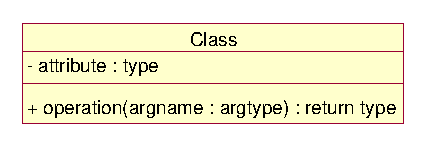
\includegraphics{umlClassIcon.eps}
        \caption{The class icon in UML.}
        \label{fig:umlClassIcon}
    \end{center}
\end{figure}
This icon is shown in Fig.~\ref{fig:umlClassIcon}.  A class icon is
simply a rectangle divided into three compartments. The topmost
show every attribute and operation of a class on any diagram.
\begin{figure}[htb]
    \begin{center}
        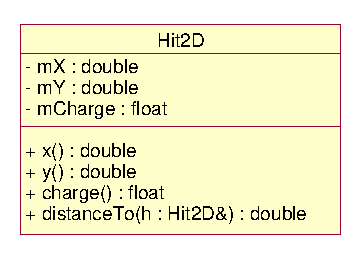
\includegraphics{umlClass.eps}
        \caption{Hit2D class. Attributes and operations are shown.}
    \end{center}
\end{figure}
Fig.~\ref{fig:umlClass} shows a typical UML description of a class
that represents a Hit (here fictitious Hit2D).  Notice that each
operations shown in italics indicate that they are pure virtual.
The corresponding C++ code for the Hit3D class from
be omitted. Notice also that the return values follow the member
functions in a similar fashion. Again, these can be omitted. Finally,
notice that the member function arguments also have a name and type.
Again one can omit the name or the arguments altogether.

At the beginning of each attribute and operations the visibility of
the class is indicated through a simple tag. UML provides three tags:
\begin{description}
\item[+] public
\item[\#] protected
\item[--] private
\end{description}
These abbreviations match exactly the three levels of visibility
provided in C++. The class shown in Fig.~\ref{fig:umlClass} is then
translated into C++ code as follows:

{\footnotesize
\begin{verbatim}
class Hit2D {
public:
Fig.~\ref{fig:umlAggregation} shows an \emph{aggregation} relationship.
    double distanceTo(Hit2D& h);
private:
    double mX, mY;
    float  mCharge;
};
\end{verbatim}
}%\footnotesize

\subsection{Composition Relationships}

Each instance of type Hit usually contains an instance of type
Position. One also says the Hit \emph{has} a Position. This is a
relationship known as composition. It can be depicted in UML using a
class relationship.  Fig.~\ref{fig:umlComposition} shows the
\emph{composition} relationship.
\begin{figure}[htb]
    \begin{center}
        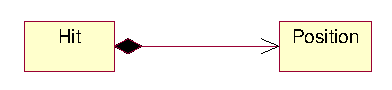
\includegraphics{umlComposition.eps}
        \caption{Class Hit has a Position.}
        \label{fig:umlComposition}
    \end{center}
\end{figure}
The black diamond represents composition. It is placed on the Hit
class because it is the Hit that is composed of (or has) a Position.
The arrowhead on the other end of the relationship denotes that the
relationship is navigable in only one direction. That is, Position
does not know about Hit. In UML relationships are presumed to be
bidirectional unless the arrowhead is present to restrict them.
Composition relationships are a strong form of containment or
aggregation. Aggregation is a whole/part relationship. In this case,
Hit is the whole, and Position is part of Hit. However, composition is
more than just aggregation. Composition also indicates that the
lifetime of Position is dependent upon Hit. This means that if Hit is
destroyed, Position will be destroyed with it.  In C++ we would
represent this as:

{\footnotesize
\begin{verbatim}
class Hit {
     Position mPos;
};
\end{verbatim}
}%\footnotesize

In this case we have represented the composition relationship as a
member variable. We could also have used a pointer so long as the
destructor of Hit deleted the pointer.  A more realistic example can
be found in \StEvent. There the \name{StHit} class has a member of
type \name{StThreeVector} which represents a position.

\subsection{Inheritance}

The inheritance relationship in UML is depicted by a triangular
arrowhead which points to the base class. One or more lines proceed
from the base of the arrowhead connecting it to the derived classes.
\begin{figure}[htb]
    \begin{center}
        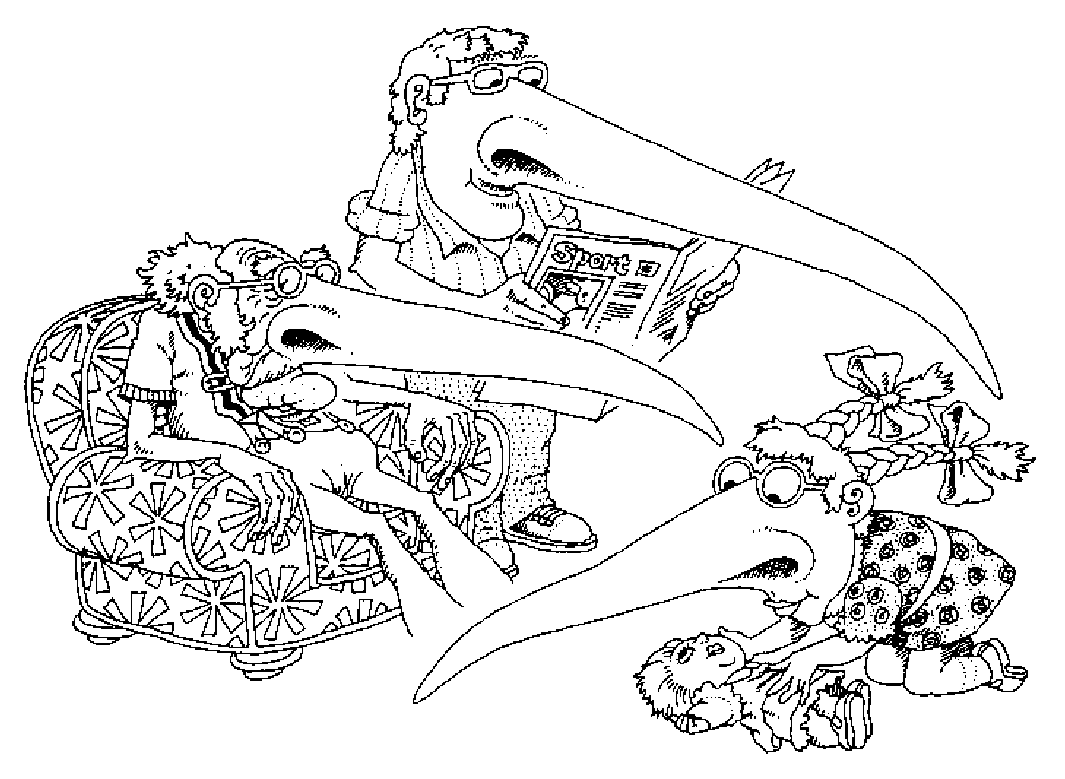
\includegraphics[width=0.7\textwidth]{cartoon6.eps}
        \caption{A subclass may inherit the structure and behaviour
            of its superclass.}
    \end{center}
\end{figure}
\begin{figure}[htb]
    \begin{center}
        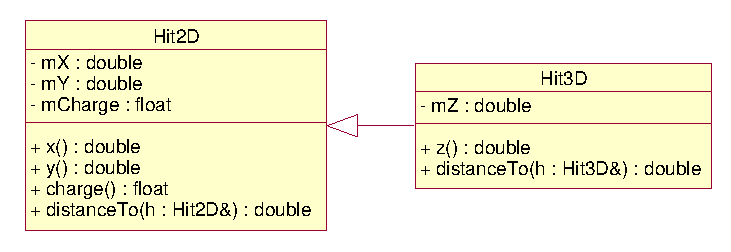
\includegraphics{umlInheritance.eps}
        \caption{Inheritance.}
        \label{fig:umlInheritance}
    \end{center}
\end{figure}

Fig.~\ref{fig:umlInheritance} shows the form of the \emph{inheritance}
relationship.  In this diagram we see that Hit3D is derived from
Hit2D.  If the name of a class would be shown in italics, it would
TrackFitter class and the CalibrartionDB class. This is the \emph{dependency}
relationship. This is often called a \emph{using} relationship.  This
relationship simply means that TrackFitter somehow depends upon
CalibrartionDB. In C++ this almost always results in a \#include:
{\footnotesize
\begin{verbatim}
class Hit3D : public Hit2D {
public:
    double z();
    double distanceTo(Hit3D& h);
private:
    double mZ;
};
\end{verbatim}
}%\footnotesize

\subsection{Aggregation and Association}

The weak form of aggregation is denoted with an open diamond. This
relationship denotes that the aggregate class (the class with the
white diamond touching it) is in some way the "whole", and the other
class in the relationship is somehow "part" of that whole.
Fig.~\ref{fig:umlAggregation} shows an \emph{aggregation}
relationship.
\begin{figure}[htb]
    \begin{center}
        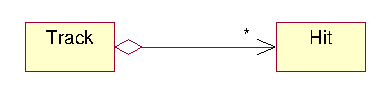
\includegraphics{umlAggregation.eps}
        \caption{Aggregation.}
        \label{fig:umlAggregation}
    \end{center}
\end{figure}
In this case, the Track class contains many Hit instances. In UML the
ends of a relationship are referred to as its "roles''. Notice that
the role at the Hit end of the aggregation is marked with a "$*$".
This indicates that the Track contains many Hit instances.  The
following Listing shows how Fig.~\ref{fig:umlAggregation} might be
implemented in C++ as:

{\footnotesize
\begin{verbatim}
class Track {
public:
    // ...
private:
    vector<Hit*> mHits;
};
\end{verbatim}
}%\footnotesize

There are other forms of containment that do not have whole/part
implications. For example, each \name{Vertex} refers back to its
parent Track. This is not aggregation since it is not reasonable to
consider a parent Track to be part of a child Vertex. We use the
\emph{association} relationship to depict this.

\begin{figure}[htb]
    \begin{center}
        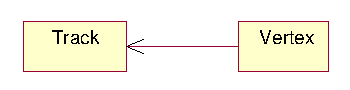
\includegraphics{umlAssociation.eps}
        \caption{Association.}
        \label{fig:umlAssociation}
    \end{center}
\end{figure}

Fig.~\ref{fig:umlAssociation} shows how we draw an association.  An
association is nothing but a line drawn between the participating
classes. In Fig.~\ref{fig:umlAssociation} the association has an
arrowhead to denote that Track does not necessarily know anything
about Vertex. This relationship will almost certainly be implemented
with a pointer of some kind.

What is the difference between an aggregation and an association?
Aggregation denotes whole/part relationships whereas associations do
not. However, there is not likely to be much difference in the way
that the two relationships are implemented.  That is, it would be very
difficult to look at the code and determine whether a particular
relationship ought to be aggregation or association.  Aggregation and
Association both correspond to the \emph{has-by-reference}
relationship.

\subsection{Dependency}

Sometimes the relationship between a two classes is very weak. They
are not implemented with member variables at all. Rather they might be
implemented as member function arguments.

Consider, for example, the fit function of a TrackFitter class.
Suppose that this function takes an argument of type CalibrartionDB
since it requires information from it (e.g. if the magnetic field was
on or off) in order to perform the fit.
\begin{figure}[htb]
    \begin{center}
        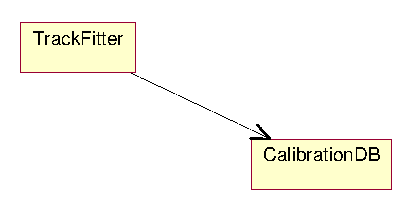
\includegraphics{umlDependency.eps}
        \caption{Dependency.}
        \label{fig:umlDependency}
    \end{center}
\end{figure}
Fig.~\ref{fig:umlDependency} shows a dashed arrow between the
TrackFitter class and the CalibrartionDB class. This is the
\emph{dependency} relationship. This is often called a \emph{using}
relationship.  This relationship simply means that TrackFitter somehow
depends upon CalibrartionDB. In C++ this almost always results in a
\#include:

{\footnotesize
\begin{verbatim}
#include "CalibrartionDB.hh"
class TrackFitter {
public:
    // ...
    void fit(CalibrartionDB &db);
private:
    // ...
};
\end{verbatim}
}%\footnotesize

%%%%%%%%%%%%%%%%%%%%%%%%%%%%%%%%%%%%%%%%%%%%%%%%%%%%%%%%%%%%%%%%%%%%
%
% The End
%
%%%%%%%%%%%%%%%%%%%%%%%%%%%%%%%%%%%%%%%%%%%%%%%%%%%%%%%%%%%%%%%%%%%%

\printindex

\end{document}
\bye
% The text following after this line is not included into the text

%
%  Template for reference section
%

%%%%%%%%%%%%%%%%%%%%%%%%%%%%%%%%%%%%%%%%%%%%%%%%%%%%%%%%%%%%%%%%%%%%
%
%    Reference: className
%
%%%%%%%%%%%%%%%%%%%%%%%%%%%%%%%%%%%%%%%%%%%%%%%%%%%%%%%%%%%%%%%%%%%%
\subsection{className}
\index{className|textbf}
\label{sec:className}
\begin{Entry}
\item[Summary]

\item[Synopsis]
    \verb+#include "className.hh"+\\
    \verb+class className;+\\

\item[Description]

\item[Persistence]
    None

\item[Related Classes]

\item[Public\\ Constructors]

\item[Public Member\\ Functions]

\item[Public Member\\ Operators]

\item[Public Functions]

\item[Public Operators]

\item[Examples]
{\footnotesize
\begin{verbatim}
//
//  What the example does
//

\end{verbatim}
}%footnotesize

\end{Entry}
